%PREAMBLE
\begin{comment}
%\documentclass[11pt]{article}
%\newcommand{\pablo}[1]{\textcolor{blue}{{\bf  #1}}}
\newcommand{\carlos}[1]{\textcolor{red}{{\bf  #1}}}
\newcommand{\fabio}[1]{\textcolor{purple}{{\bf  #1}}}
\newcommand{\susana}[1]{\textcolor{violet}{{\bf  #1}}}

% HEP names :: https://ctan.javinator9889.com/macros/latex/contrib/hepnames/hepnames.pdf

\DeclarePairedDelimiter\bra{\langle}{\rvert}
\DeclarePairedDelimiter\ket{\lvert}{\rangle}
\DeclarePairedDelimiterX\braket[2]{\langle}{\rangle}{#1 \delimsize\vert #2}

\newcommand*{\yt}{\ensuremath{y_{t}}\xspace}
\newcommand*{\tchannel}{\ensuremath{t\text{-channel}}\xspace}
\newcommand*{\schannel}{\ensuremath{s\text{-channel}}\xspace}
%\newcommand*{\lepT}{\ensuremath{\Pl_{\Pt}}\xspace}
%\newcommand*{\lepH}{\ensuremath{\Pl_{\PHiggs}}\xspace}

%\newcommand*{\muR}{\ensuremath{\mu_{\text{R}}}\xspace}
%\newcommand*{\muF}{\ensuremath{\mu_{\text{F}}}\xspace}

% Add external packages
\usepackage[italic]{hepnicenames}

%%%%%%%%%%%%%%%%%%%%%%%
%  From NA-HIGG-2020-02-INT1-defs.sty    %
%%%%%%%%%%%%%%%%%%%%%%%
% Basic tHq-related macros
%\newcommand*{\tHq}{\ensuremath{\Pqt{}\PH{}\Pq}\xspace}
%\newcommand*{\tHq}{\ensuremath{\Ptop \PHiggs \Pq}\xspace}
%\newcommand*{\tHq}{\Pqt{}\PH{}\Pq}
\newcommand*{\tHq}{\ensuremath{tHq}\xspace}
\newcommand*{\tH}{\ensuremath{\Pqt{}\PH{}}\xspace}
\newcommand*{\tHqsec}{\texorpdfstring{\Pqt{}\PH{}\Pq}{tHq}}
\newcommand*{\tHqML}{\ensuremath{\Pqt{}\PH{}\Pq\,(\text{ML})}\xspace}
\newcommand*{\tHqbb}{\ensuremath{\Pqt{}\PH{}\Pq\,(\bbbar)}\xspace}
\newcommand*{\tbarHq}{\Paqt{}\PH{}Pq}
\newcommand*{\tHbb}{\ensuremath{\tHq (\PH \to \bbbar)}\xspace}
\newcommand*{\tHtautau}{\ensuremath{\tHq (\PH \to \Pgt{}\Pgt)}\xspace}
\newcommand*{\dR}{\ensuremath{\Delta R}\xspace}
\newcommand*{\trexfitter}{TRExFitter\xspace}
\newcommand*{\thqloop}{\texttt{tHqLoop}\xspace}


\newcommand*{\MpT}{\ensuremath{\vec{p}_{\text{T}}^{\text{miss}}}\xspace}
\newcommand*{\mtw}{\ensuremath{m_{\text{T}}(\Pl,\MET)}}
\newcommand*{\mlb}{\ensuremath{m_{\Pl\Pqb}}}
\newcommand*{\mOSSF}{\ensuremath{m_{\text{OSSF}}}\xspace}

% Background processes
\newcommand*{\ttX}{\ensuremath{\Pqt{}\Paqt{}X}\xspace}
\newcommand*{\tX}{\ensuremath{\Pqt{}X}\xspace}

%\newcommand*{\ttX}{\Pqt{}\Paqt{}+X}
\newcommand*{\ttH}{\Pqt{}\Paqt{}\PH}
%\newcommand*{\ttH}{\ensuremath{\Pqt{}\Paqt{}\PH}\xspace}
\newcommand*{\ttZ}{\Pqt{}\Paqt{}\PZ}
\newcommand*{\ttV}{\ensuremath{\Pqt{}\Paqt{}V}\xspace}
\newcommand*{\ttW}{\Pqt{}\Paqt{}\PW}
\newcommand*{\ttWj}{\ensuremath{t\bar{t}W+j}\xspace}
\newcommand*{\tZq}{\Pqt{}\PZ{}\Pq}
\newcommand*{\tWZ}{\Pqt{}\PW{}\PZ}
\newcommand*{\tWH}{\Pqt{}\PW{}\PH}
\newcommand*{\tHW}{\Pqt{}\PW{}\PH}
\newcommand*{\tW}{\Pqt{}\PW}
\newcommand*{\Wt}{\Pqt{}\PW}
\newcommand*{\diboson}{diboson\xspace}
\newcommand*{\Diboson}{Diboson\xspace}
\newcommand*{\triboson}{triboson\xspace}
\newcommand*{\Triboson}{Triboson\xspace}
\newcommand*{\Vjets}{\ensuremath{V\text{+\,jets}}\xspace}

\newcommand*{\ttt}{\ensuremath{ttt}\xspace}
\newcommand*{\tttt}{\ensuremath{t\bar{t}t\bar{t}}\xspace}
\newcommand*{\ggH}{\ensuremath{ggH}\xspace}
\newcommand*{\qqH}{\ensuremath{qqH}\xspace}
\newcommand*{\WH}{\ensuremath{WH}\xspace}
\newcommand*{\ZH}{\ensuremath{ZH}\xspace}

% Fake leptons
\newcommand*{\elHF}{\ensuremath{e_{\text{HF}}}\xspace}
\newcommand*{\muHF}{\ensuremath{\mu_{\text{HF}}}\xspace}
\newcommand*{\elCo}{\ensuremath{e_{\text{conv}}}\xspace} 
\newcommand*{\kelHF}{\ensuremath{\mu(e_{\text{HF}})}\xspace}
\newcommand*{\kmuHF}{\ensuremath{\mu(\mu_{\text{HF}})}\xspace}
\newcommand*{\kelCo}{\ensuremath{\mu(e_{\text{conv}})}\xspace} 

% Signal regions
\newcommand*{\dileptau}{\ensuremath{2\Pl+1\tauhad}\xspace}
\newcommand*{\dilepOStau}{\ensuremath{2\Pl\,\text{OS}+1\tauhad}\xspace}
\newcommand*{\dilepSStau}{\ensuremath{2\Pl\,\text{SS}+1\tauhad}\xspace}

\newcommand*{\onelep}{\ensuremath{1\Pl}\xspace}
\newcommand*{\dilep}{\ensuremath{2\Pl}\xspace}
\newcommand*{\dilepOS}{\ensuremath{2\Pl\,\text{OS}}\xspace}
\newcommand*{\dilepSS}{\ensuremath{2\Pl\,\text{SS}}\xspace}
%\newcommand*{\SS}{\ensuremath{\text{SS}}\xspace}
%\newcommand*{\OS}{\ensuremath{\text{OS}}\xspace}

\newcommand*{\trilep}{\ensuremath{3\Pl}\xspace}
\newcommand*{\lepditau}{\ensuremath{1\Pl+2\tauhad}\xspace}




\newcommand*{\lumi}{\ensuremath{\mathcal{L}}\xspace}
\newcommand*{\lumiunits}{$\,$ cm$^{2} \,$s$^{-1}$\xspace}


%Other
\newcommand*{\CM}{\ensuremath{\sqrt{s}}\xspace}
 
\newcommand*{\Wtb}{\ensuremath{tWb}\xspace}
\newcommand*{\tWb}{\Wtb}
%\newcommand*{\tWb}{\ensuremath{tWb}\xspace}
\newcommand*{\pfour}{\ensuremath{\boldsymbol{\textrm{p}}}\xspace} 

\newcommand*{\tchan}{\ensuremath{t}-channel}
\newcommand*{\mtop}{\ensuremath{m_{\Ptop}}\xspace}
%\newcommand*{\mH}{\ensuremath{m_H}\xspace}
%\newcommand*{\HT}{\ensuremath{H_{\text{T}}}\xspace}

%\newcommand*{\PWplus}{\ensuremath{\PW^{+}}\xspace}
%\newcommand*{\PWminus}{\ensuremath{\PW^{-}}\xspace}
%\newcommand*{\Pgamma}{\ensuremath{\gamma}\xspace}

 \newcommand*{\greekphys}{\ensuremath{\varphi\upsilon\sigma\iota\kappa \eta}\xspace}
 \newcommand*{\greekatom}{\ensuremath{\alpha \tau o \mu o \nu}\xspace}
 \newcommand{\emu}{\ensuremath{\Pe/\Pmu}\xspace}

\newcommand*{\momentum}{\ensuremath{\overrightarrow{p}}\xspace} 
%\newcommand*{\CP}{\ensuremath{\mathcal{CP}}\xspace}
\newcommand*{\CP}{CP\xspace}

% Decays (Please, check latex/atlasprocess.sty and latex/atlasparticle.sty for more definitions!)
\newcommand{\bb}{\ensuremath{\Pqb\Paqp}\xspace}
\newcommand{\WW}{\ensuremath{\PW\PW^{*}}\xspace}
\newcommand{\ZZ}{\ensuremath{\PZ\PZ^{*}}\xspace}
\newcommand{\Higgsdecays}{\ensuremath{\PH \rightarrow b\bar{b}, \WW, \ZZ, \tau\tau}\xspace}
\newcommand{\Higgsdecayslep}{\ensuremath{\PH \rightarrow \WW, \ZZ, \tau\tau}\xspace}
\newcommand{\HWW}{\ensuremath{\PH \rightarrow \WW}\xspace}
\newcommand{\HZZ}{\ensuremath{\PH \rightarrow \ZZ}\xspace}

% reconstruction definitions
\newcommand{\pnutop}{\ensuremath{\vec{p^{\Pnu, \text{top}}}}\xspace}
\newcommand{\pnutopx}{\ensuremath{p^{\Pnu, \text{top}}_x}\xspace}
\newcommand{\pnutopy}{\ensuremath{p^{\Pnu, \text{top}}_y}\xspace}
\newcommand{\pnutopz}{\ensuremath{p_{z}(\Pnu_{\text{top}})}\xspace}
\newcommand{\pnutopT}{\ensuremath{\pT(\Pnu_{\text{top}})}\xspace}
\newcommand{\phinutop}{\ensuremath{\phi(\Pnu_{\text{top}})}\xspace}
\newcommand{\pltop}{\ensuremath{\vec{p^{\Plepton, \text{top}}}}\xspace}
\newcommand{\pltopx}{\ensuremath{p^{\Plepton, \text{top}}_x}\xspace}
\newcommand{\pltopy}{\ensuremath{p^{\Plepton, \text{top}}_y}\xspace}
\newcommand{\pltopz}{\ensuremath{p^{\Plepton, \text{top}}_z}\xspace}
\newcommand{\pltopT}{\ensuremath{\pT(\Plepton_{\text{top}})}\xspace}
\newcommand{\philtop}{\ensuremath{\phi(\ell_{\text{top}})}\xspace}
\newcommand{\phibtop}{\ensuremath{\phi(b_{\text{top}})}\xspace}
\newcommand{\tauvis}{\ensuremath{\Ptau_{\text{vis}}}\xspace}

\newcommand{\leptop}{\ensuremath{\Plepton^{\text{top}}}\xspace}
\newcommand{\lepH}{\ensuremath{{\Plepton^{\PH}}}\xspace}
\newcommand{\Hvismass}{\ensuremath{m_{\PH}^{\text{vis}}}\xspace}
\newcommand{\toprecomass}{\ensuremath{\mtop^{\text{reco}}}\xspace}
% \newcommand{\toprecomass}{\ensuremath{\Pqt_{\text{reco}}^{\text{m}}\xspace}}
% \newcommand{\Hvismass}{\ensuremath{\PH_{\text{vis}}^{\text{m}}\xspace}}
\newcommand{\MMC}{\texttt{MissingMassCalculator}\xspace}

% luminosity (2015)
\newcommand{\lumiFifteenRelUnc}{1.13} % in [%]
\newcommand{\lumitagFifteen}{{\small\texttt{OfLumi-13TeV-008}}}
%\newcommand{\lumiFifteenInPbNoUnits}{3219.56}
%\newcommand{\lumiFifteenInFbNoUnits}{3.2}
\newcommand{\lumiFifteenInPbNoUnits}{3244.54} % final luminosity recommendation for Run 2 analyses (https://twiki.cern.ch/twiki/bin/viewauth/Atlas/LuminosityForPhysics#2015_2018_13_TeV_proton_proton_f)
\newcommand{\lumiFifteenInFbNoUnits}{3.2}
%\newcommand{\dataperiodsFifteen}{D--J}
\newcommand{\dataperiodsFifteen}{D--H,J}
\newcommand{\firstdatarunFifteen}{276262}
\newcommand{\lastdatarunFifteen}{284484}
\newcommand{\datarunsFifteen}{\firstdatarunFifteen--\lastdatarunFifteen}
\newcommand{\dataeventsFifteen}{220.58M}

% luminosity (2016)
\newcommand{\lumiSixteenRelUnc}{0.89} % in [%]
\newcommand{\lumitagSixteen}{{\small\texttt{OfLumi-13TeV-009}}}
%\newcommand{\lumiSixteenInPbNoUnits}{32988.1}
%\newcommand{\lumiSixteenInFbNoUnits}{33.0}
% final luminosity recommendation for Run 2 analyses (https://twiki.cern.ch/twiki/bin/viewauth/Atlas/LuminosityForPhysics#2015_2018_13_TeV_proton_proton_f)
\newcommand{\lumiSixteenInPbNoUnits}{33402.2}
\newcommand{\lumiSixteenInFbNoUnits}{33.4}
%\newcommand{\dataperiodsSixteen}{A--L}
\newcommand{\dataperiodsSixteen}{A--G,I,K,L}
\newcommand{\firstdatarunSixteen}{297730}
\newcommand{\lastdatarunSixteen}{311481}
\newcommand{\datarunsSixteen}{\firstdatarunSixteen--\lastdatarunSixteen}
\newcommand{\dataeventsSixteen}{1057.84M}

% luminosity (2017)
\newcommand{\lumiSeventeenRelUnc}{1.13} % in [%]
\newcommand{\lumitagSeventeen}{{\small\texttt{OfLumi-13TeV-010}}}
%\newcommand{\lumiSeventeenInPbNoUnits}{44307.4}
%\newcommand{\lumiSeventeenInFbNoUnits}{44.3}
% final luminosity recommendation for Run 2 analyses (https://twiki.cern.ch/twiki/bin/viewauth/Atlas/LuminosityForPhysics#2015_2018_13_TeV_proton_proton_f)
\newcommand{\lumiSeventeenInPbNoUnits}{44630.6}
\newcommand{\lumiSeventeenInFbNoUnits}{44.6} 
%\newcommand{\dataperiodsSeventeen}{B--K}
\newcommand{\dataperiodsSeventeen}{B--F,H,I,K}
\newcommand{\firstdatarunSeventeen}{325713}
\newcommand{\lastdatarunSeventeen}{340453}
\newcommand{\datarunsSeventeen}{\firstdatarunSeventeen--\lastdatarunSeventeen}
%%%\newcommand{\datarunsSeventeen}{324320--341649}
\newcommand{\dataeventsSeventeen}{1340.80M}

% luminosity (2018)
\newcommand{\lumiEightteenRelUnc}{1.10} % in [%]
\newcommand{\lumitagEightteen}{{\small\texttt{OfLumi-13TeV-010}}}
%\newcommand{\lumiEightteenInPbNoUnits}{58450.1}
%\newcommand{\lumiEightteenInFbNoUnits}{58.5}
% final luminosity recommendation for Run 2 analyses (https://twiki.cern.ch/twiki/bin/viewauth/Atlas/LuminosityForPhysics#2015_2018_13_TeV_proton_proton_f)
\newcommand{\lumiEightteenInPbNoUnits}{58791.6}
\newcommand{\lumiEightteenInFbNoUnits}{58.8}
\newcommand{\lumiEightteenInPb}{\SI{\lumiEightteenInPbNoUnits}{\per\pb}}
\newcommand{\lumiEightteenInFb}{\SI{\lumiEightteenInFbNoUnits}{\per\fb}}
%\newcommand{\dataperiodsEightteen}{B--Q}
\newcommand{\dataperiodsEightteen}{B--D,F,I,K,L,M,O,Q}
\newcommand{\firstdataruEightteen}{348885}
\newcommand{\lastdatarunEightteen}{364292}
\newcommand{\datarunsEightteen}{\firstdataruEightteen--\lastdatarunEightteen}
%%%\newcommand{\datarunsEightteen}{348197--364292}
\newcommand{\dataeventsEightteen}{1716.77M}

% luminosity (2015+2016+2017)
%\newcommand{\lumiInPb}{80515.06~\invpb}
% \newcommand{\partlumi}{\SI{80.52}{\per\fb}}
%\newcommand{\datafirstyear}{2015}
%\newcommand{\datalastyear}{2017}

% luminosity (2015+2016+2017+2018)
%
% https://twiki.cern.ch/twiki/bin/viewauth/Atlas/LuminosityForPhysics#2015_2018_13_TeV_proton_proton_f
% final luminosity recommendation for Run 2 analyses (central value + uncertainty)
\newcommand{\lumiRelUnc}{0.83} % in [%]
\newcommand{\lumiInPbNoUnits}{140068.94} % in pb-1
\newcommand{\lumiInFbNoUnits}{140} % in fb-1
\newcommand{\lumiWithUnc}{\ensuremath{140.1 \pm 1.2}\,\si{\per\fb}} % in fb-1
%
% old recommendation
%\newcommand{\lumiRelUnc}{1.7} % in [%]
%\newcommand{\lumiInPbNoUnits}{138965.16} % in pb-1
%\newcommand{\lumiInFbNoUnits}{139} % in fb-1
%\newcommand{\lumiWithUnc}{\ensuremath{\lumiInFbNoUnits \pm 2.4}\,\si{\per\fb}} % in fb-1
\newcommand{\dataeventsAll}{4335.99M}
%
\newcommand{\lumiInPb}{\SI{\lumiInPbNoUnits}{\per\pb}}
%\newcommand{\lumi}{\SI{\lumiInFbNoUnits}{\per\fb}}
\newcommand{\datafirstyear}{2015}
\newcommand{\datalastyear}{2018}

% % tunes and PDF sets
\def\cteq{CTEQ6L1\xspace}
\def\ctten{CT10\xspace}
\def\cttennlo{CT10\,NLO\xspace}
\def\cttennnlo{CT10\,NNLO\xspace}
\def\ctfourteennlo{CT14\,NLO\xspace}
\def\ctfourteennnlo{CT14\,NNLO\xspace}
\def\nnpdfnnlo{NNPDF3.0\,NNLO\xspace}
\def\nnpdfnlofourflav{NNPDF3.0\,NLO\,nf4\xspace}
\def\nnpdfnlo{NNPDF3.0\,NLO\xspace}
\def\nnpdftwonlo{NNPDF2.3\,NLO\xspace}
\def\nnpdftwo{NNPDF2.3\,LO\xspace}
\def\nnpdftwofiveflav{NNPDF2.3\,5f\,FFN\xspace}
\def\mstw{MSTW2008\,NLO\xspace}
\def\a14{A14\xspace}
\def\auet{AUET2\xspace}
\def\aznlo{AZNLO\xspace}
\def\mmhtnnlo{MMHT2014\,NNLO\xspace}
\def\mmhtnlo{MMHT2014\,NLO\xspace}
\def\mmhtlo{MMHT2014\,LO\xspace}
\def\mstwnlo{MSTW2008\,68\%\,CL\,NLO \xspace}
\def\mstwnnloninety{MSTW2008\,90\%\,CL\,NNLO \xspace}
\def\ueee{UE-EE-5\xspace}




 
\endinput


%\begin{document}
asdf
%ENDPREAMBLE
\end{comment}

\chapter{Recording data and simulating events with the ATLAS detector}
%{\LARGE \textbf{}\\}
% The content of this section has to be general, i.e. it is valid for both the polarisation and the tHq analyses
%\tableofcontents
\label{chap:DataAndMC}

\vspace*{0.1 cm} 
\hspace*{200pt} \\
\hspace*{120pt} \textit{In God we trust, all others bring data.} \\
%\hspace*{200pt} \textit{} \\
%\hspace*{200pt} \\
\hspace*{140pt} ---\textsc{William Edwards Deming (1900-1993)} \\% \textit{} \\
%\hspace*{200pt} \textit{Please check your e-mailing list} \\
\vspace*{2cm} 


In particle physics, $\Pproton \Pproton$ collisions are studied to improve our understanding 
of physics of the elementary particles and their interactions. The LHC provides these collisions 
and the ATLAS detector records them. 
In order to allow a statistical interpretation of the collision data, the theoretical prediction is 
derived making use of Monte Carlo (MC) generators.\footnote{The scientific method is to compare the prediction 
and the collected data. Then, if there is a disagreement, one needs to update the model that produced the prediction. 
This procedure is done iteratively.}.  The current baseline theory to describe
%maybe remove footnote
the interactions between particles is the SM.
%This theory is simulated via Monte Carlo (MC) generators %which calculate the hard interaction 
%in $\Pproton \Pproton$ collisions and the subsequent evolution in the parton-shower, and the hadronisation. 
%Subsequently, the detector response is simulated to be able to compare to the real-collision data. 




%The word ``event'' is among the most commonly used terms in high-energy physics.
%In the context of the LHC experiments there are two types of events. On the one side, there
%are the authentic data events recorded by the detector. This event is typically a 
%$\Pproton \Pproton$ collision but it could also be a single particle such as
%cosmic ray. On the other side, there are the events simulated by the different 
%event generators based on Monte Carlo (MC) methods. 
%In the ATLAS experiment, both type of events are processed by a common
%software.
For real-collision data, the detector response is evaluated via various algorithms
in order to reconstruct the objects in the final state.
For the simulated processes,
the MC-generated particles undergo a series of steps replicating the physics of
the collisions, the interaction with the detector material, the magnetic fields, and
the response of the detector and its electronics. Once these steps are applied,
the simulated events are processed using the same algorithms as the ones 
used with real-collision data. 


 This chapter is divided into three sections: In Section~\ref{sec:Chap2:PhenoOfPP}, the phenomenology of 
 the $\Pproton \Pproton$ collisions is described. Here the parton model and underlying
 event are presented. The concepts of luminosity and pile-up are discussed as well.
% In the other two sections, the two types of data described above, 
 %the real and the simulated, are detailed.
Section~\ref{sec:Chap3.1:Data} describes the collection of the 
 data with the ATLAS detector, while Section~\ref{sec:Chap3.1:MC}
 discusses the generation of simulated data by presenting the steps and tools
 of the simulation chain.


%%%%%%%%%%%%%%
%          PP Collisions        %
%%%%%%%%%%%%%%
\section{Phenomenology of proton--proton collisions}
\label{sec:Chap2:PhenoOfPP}


The analysis presented in this thesis uses data obtained from $\Pproton\Pproton$ collisions 
provided by the LHC.
Therefore, understanding the physics behind these collisions is fundamental to understanding the physics
analyses conducted at this collider.
The $\Pproton\Pproton$ collisions can be categorised into two broad classes based on how 
the energy and momentum are distributed among the colliding particles. Collisions can be elastic and inelastic.
In the former, the kinetic energy is conserved and the collision is a scattering off 
two protons without changing their intrinsic properties or producing any new particles.
In the latter, the protons either change their intrinsic properties or new particles
are produced as the result of the collision.

%At the LHC energy regime, $\Pproton \Pproton$ collisions cannot be
%described as a point-like interactions. Since the collision energy is so high,
%the inelastic collisions regime dominates the physics by several orders 
At the LHC energy regime, the $\Pproton \Pproton$ collisions are predominantly
inelastic and they cannot be described as point-like interactions.
Here is where the parton model and the PDFs come into play.
The PDFs are functions containing the long-distance structure of the hadrons in 
terms of valence and sea quarks and gluons (explained in Section~\ref{sec:Chap2:PhenoOfPP:ProtonStructure}). 
%More information about PDFs and the proton structure can be found in Section~\ref{sec:Chap2:PhenoOfPP:ProtonStructure}.
This description is known as the ``parton model'' and is discussed throughout this section.

During the Run~2 data-taking period of the LHC, $\Pproton\Pproton$ collisions took place with a centre-of-mass 
energy of $13$~TeV. The total cross-section of $\Pproton\Pproton$ collisions at this energy is measured to 
be $\sigma_{\text{tot}} = (110.6 \pm 3.4)$~mb~\cite{Cafagna:2021sge}. The method used to measure $\sigma_{\text{tot}}$ also made it 
possible to separate the cross-section into the elastic $\sigma_{\text{el}} = (31.9 \pm 1.7)$~mb and 
the inelastic one $\sigma_{\text{inel}} = (79.5 \pm 1.8)$~mb.
%The inelastic cross-section is the sum of the non-diffractive and the diffractive cross-section. 
However, only inelastic scattering generates particles with a sufficient angle with respect to the beam 
axis so that these particles enter into the geometrical acceptance of the detector. 
%Figure~\ref{fig:Chap2:pp_cross_section_pdg} shows the cross-section (elastic, inelastic and total) for $\Pproton \Pproton$ collisions depending on \CM.
The cross-section can be computed as the convolution of PDFs with the parton 
scattering matrix element $\mathcal{M}$. 
In the context of scattering experiments, the $\mathcal{M}$ refers to the amplitude 
for a particular scattering or decay process between initial and final states. 
The $\mathcal{M}$ provides information about the probability of transitioning 
from an initial state to a final state through a given interaction.

%(the matrix element,$\mathcal{M}$, was already introduced in Section~\ref{sec:Chap1:tH}).

%\begin{figure}[h]
% 	 \centering
% 	  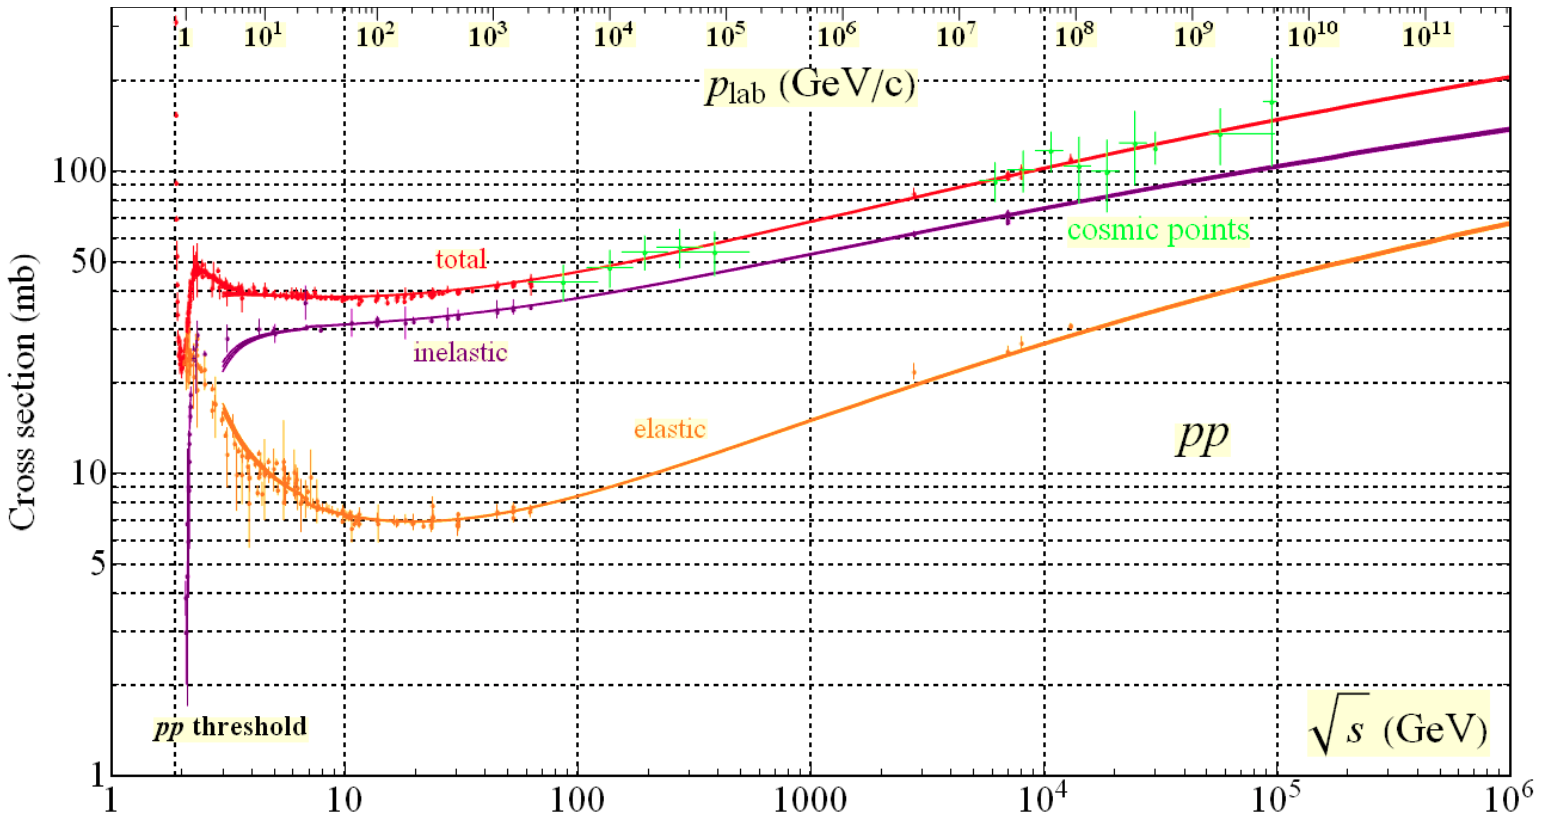
\includegraphics[width = 0.75\textwidth]{Chapter2/pp_cross_section_pdg}
%	  \caption{Total and elastic cross-section for $\Pproton \Pproton$ collisions as a 
%	  		function of the laboratory momentum and the $\CM$~\cite{pdgXsecProton}.
%			At $\CM=13$~TeV, $\sigma_{\text{el}} = (31.9\pm1.7)$~m, $\sigma_{\text{inel}} = (79.5\pm1.8)$~mb and 
%			$\sigma_{\text{tot}} = (110.6\pm3.4)$~mb.} 
%	\label{fig:Chap2:pp_cross_section_pdg}% source: $~https://pdg.lbl.gov/1998/hadronicrpp_page13.pdf
%\end{figure}




%See: https://arxiv.org/pdf/1611.07864.pdf
% https://indico.cern.ch/event/760184/contributions/3290951/attachments/1832936/3002261/rojo-SMLHC-PDFrev.pdf


%%%%%%%%%%%%%%%%
%           Proton structure        %
%%%%%%%%%%%%%%%%
\subsection{Proton structure and parton model}
\label{sec:Chap2:PhenoOfPP:ProtonStructure}
%As mentioned above, the protons are not fundamental particles but
%they are composed by quarks and gluons. This description is knonw
%as parton model.
%\begin{minipage}{.45\textwidth}
%\begin{figure}
%  	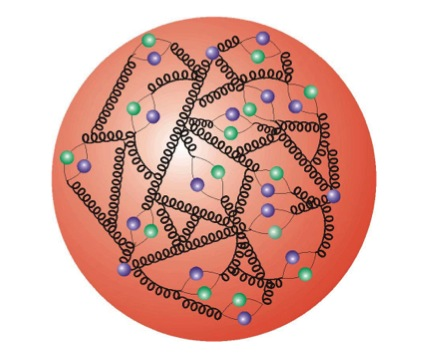
\includegraphics[width = \textwidth]{Chapter2/PartonCompositionOfHadron}
%	\caption{Content of a hadron in the parton model. For baryons like the proton there are 3 valence quarks, many virtual quark and anti-quarks pairs (sea quarks) and many gluons.}
%	\label{fig:Chap2:PartonComposition}
%\end{figure}
%\end{minipage}\hfill
%\begin{minipage}{.54\textwidth}
%\end{minipage}

Formulated by R.$\,$P. Feynman the parton model for hadrons describes these non-fundamental 
particles as a composite of several point-like constituents named partons~\cite{Feynman:1969ej}.
In this model, the proton is not only made of its three ``valence''  quarks 
(two $\Pup$-type and one $\Pdown$-type quarks) but also, there is a ``sea'' of
gluons and short-lived quark--antiquark pairs created through gluon splitting.
The partons in the sea are continuously interacting with each other and, depending
on the energy, can have any flavour.



%The parton distribution functions (PDFs) are density functions that describe probability to find a parton carrying a fraction $x$
%of the total proton momentum at a squared energy scale $Q^2$. 
%The PDFs describe the distribution of the hadron's momentum among its constituents\cite{Butterworth:2015oua}.
%The momentum distribution function of the partons within the proton is obtained by a fit on a large number of cross-section data points
%over a grid of $x$ and $Q^2$ values obtained from many experiments (deep inelastic scattering, Drell-Yan and jet measurements).
%There are various global fitting collaborations (ABM, CT, MMHT, NNPDF, MSTW, CTEQ),
%each taking different approaches to this fitting procedure. These fits are later extrapolated to new energy scales. %Several collaborations
%work on providing the PDFs sets (CT14, MMHT2014, NNPDF30, ...)
%The most relevant uncertainties associated with the computation of PDFs are the experimental uncertainties of the
%input datasets and the theoretical uncertainties of the coupling parameters. 

%Formally, the PDF $f_{a/A}(x, Q^{2})$ is defined as the probability of finding
%a parton $a$ within the hadron $A$ carrying a fraction $x=p_{a}/p_{A}$ of its momentum at $Q^{2}$ energy scale.
%The energy scale $Q$ characterises the hard scattering and typically corresponds to the momentum transfer in the given process.
%As an example, several PDFs at two different scale energies are presented in Figure~\ref{fig:Chap2:NNLO_PDF} as a function of $x$.

The distribution of the momentum of a hadron among its constituents is described by its
PDFs~\cite{Butterworth:2015oua}. The momentum of the partons within a proton is 
determined through fits to several data points obtained from experimental data 
such as the ones coming from deep inelastic scattering, Drell-Yan, and jet measurements. Various global fitting 
collaborations, including ABM~\cite{Alekhin:2013nda}, CT~\cite{Dulat:2015mca}, 
MMHT~\cite{Harland-Lang:2014zoa}, NNPDF~\cite{NNPDF:2014otw}, MSTW~\cite{Watt:2012tq}, and CTEQ~\cite{Hou:2019efy}, employ different 
methods to perform these fits, which are subsequently extrapolated to new energy scales.

Formally, the PDF $f_{a/A}(x, Q^{2})$ is the probability of finding parton $a$ in a hadron $A$ 
carrying a fraction $x=p_{a}/p_{A}$ of its momentum at the energy scale $Q^2$. 
At lower energies (i.e. $Q\sim1$~GeV), the momentum of a proton is primarily shared 
among its valence quarks, while at higher energies (i.e. $1 <Q \lesssim 1$~GeV), 
the emission of gluons carrying some of the initial momentum of the quarks is more likely.
As an example, PDFs for several parton flavours at two different energy scales as a function of $x$ 
are presented in Figure~\ref{fig:Chap2:NNLO_PDF}.
In QCD theory, these interactions can be divided into two categories: 
Hard-scattering, which can be calculated by perturbation theory due to the small $\alpha_{s}$, and 
low-energy processes, which cannot be calculated because $\alpha_{s}$ is large and 
have a much greater impact on non-perturbative QCD. 
%hard (large momentum transfer) and soft (low momentum transfer). 
%Hard-scattering processes are well understood and can be predicted with considerable precision,
%while soft interactions have a much greater impact of non-perturbative QCD and are more challenging to calculate.

\begin{figure}[h]
 	  \centering
	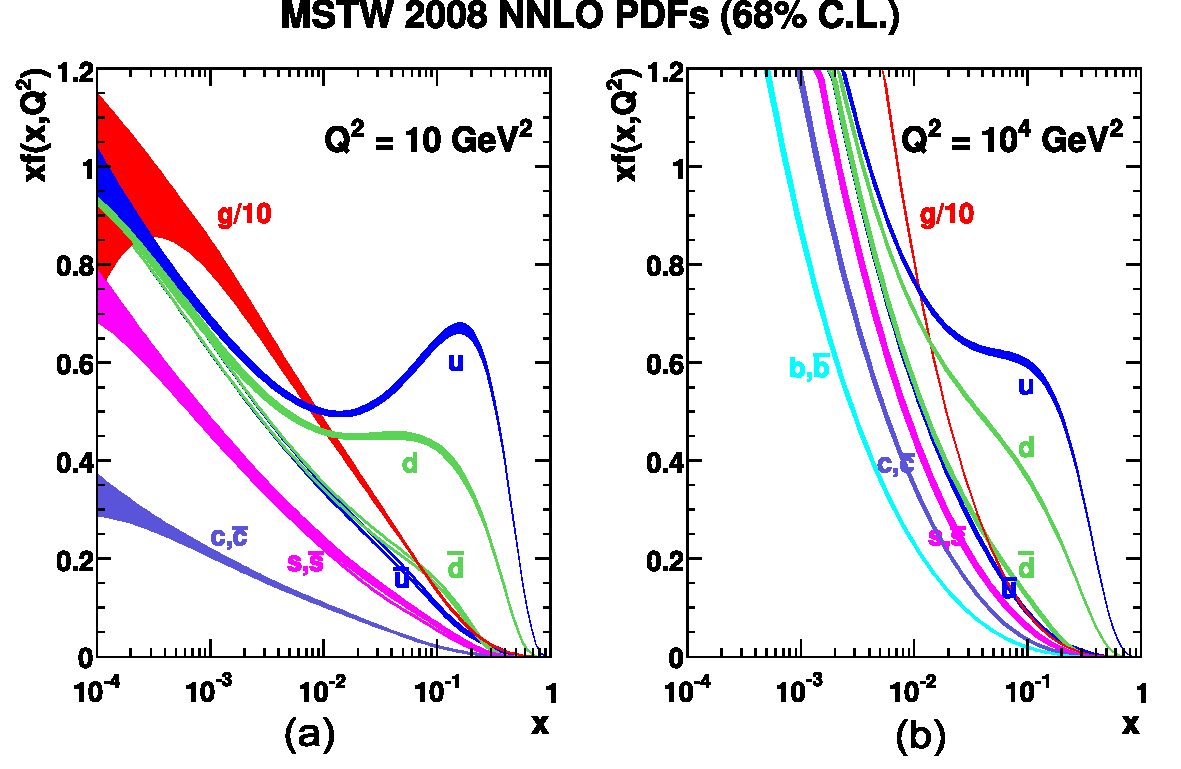
\includegraphics[width = \textwidth]{Chapter2/PDF_mstw2008nnlo68cl_allpdfs_A_B}
	\caption{Parton distribution functions $xf(x,q^{2})$ against the fraction $x$ 
		      for gluons and different quark flavours 
		      at (a) $Q^{2}=10$~GeV$^2$ and (b) $Q^{2}=10^{4}$~GeV$^2$ energy scales using the MSTW 
		      2008 NNLO PDF sets~\cite{Martin:2009iq}.}
	\label{fig:Chap2:NNLO_PDF}
\end{figure} 


%The momentum of the proton is distributed among its constituents and, while at lower energies ($Q\sim1$~GeV) it is shared mainly between the 
%valence quarks, at higher energies ($1 <Q \lesssim 1$~GeV) the emission of gluons carrying a some of the initial momentum of the quark is more probable.
%Within the QCD theory, these interactions can be classified in two main groups: ``hard'' and ``soft''. The hard processes are those involving large 
%momentum transfer.  This type of processes are well understood and their cross-section can be predicted with good precision using perturbation theory.
%In contrast, the low momentum transfer of soft interactions leads to a much more dominant impact of non-perturbative QCD, which makes much more difficult to
%calculate the cross-section. 

When two protons ($A$ and $B$) collide at the LHC, their partons can interact via a 
hard-scattering process. Each of the interactions between the parton pairs is independent 
of the interactions with other partons. The remaining partons also contribute 
to the final state as ``underlying events'' (see Section~\ref{sec:Chap1:PhenoOfPP:UE}).  
Figure~\ref{fig:Chap2:ProtonProton_Collision} provides a simplified representation of a $\Pproton \Pproton$ collision.
In this schema, each of the two partons that interact carries a different fraction $x_{i=a,b}$ of the
total proton energy.

\begin{figure}[h]
 	  \centering
	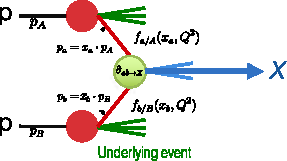
\includegraphics[width = 0.70\textwidth]{Chapter2/ProtonProton_Phenomenology_ByMe}
	\caption{Simplified view of a $\Pproton \Pproton$ collision.
		The PDFs represent the structure of the proton (red) and they are obtained using experimental 
		data and QCD properties. The light green bubble represents the hard-scatter parton cross-section. 
		The blue $X$ is the product of the interaction and it can be jets, bosons, quarks or any other particles.} 
		% Image modified from ~\cite{Hoecker:2016vvy}
	\label{fig:Chap2:ProtonProton_Collision}
\end{figure}


The total cross-section ($\sigma$) in a hadron--hadron hard-scattering process in which 
a parton $a$ from hadron $A$ interacts with a parton $b$ from 
hadron $B$, such as a $\Pproton \Pproton$ interaction, to produce a final-state $X$ is:
\begin{equation*} % Sacado de lo de Galo
	\sigma_{AB \rightarrow X} = \sum_{a, b} \iint dx_{a} dx_{b} f_{a}(x_{a}, Q^{2})  f_{b}(x_{b}, Q^{2}) \hat{\sigma}_{ab\rightarrow X}\, ,
\end{equation*}
where $f_{i}(x_{i}, Q^{2})$ is the PDF of $i = A,\, B$.
Here, the $Q$ is chosen to be the factorisation scale\footnote{The 
factorisation scale $\mu_{\text{F}}$ establishes the boundary between low and high energy,
thereby determining the scale at which perturbative calculations become valid.} ($\mu_{\text{F}}$).
The contribution of the individual partons $a$ and $b$ is denoted by  $\hat{\sigma}_{ab\rightarrow X}$.  
With this equation, all processes in $\Pproton \Pproton$ collisions can be computed. 

Depending on the order achieved in perturbation theory (LO, NLO, NNLO, ...), the cross-section 
of the individual partons to produce the final state of interest
($ab \rightarrow X$) can be calculated as:
\begin{align*}
	\hat{\sigma}_{ab\rightarrow X} 	&= \sum_{i=0}^{\infty} \alpha_{s}^{i}(\mu_{\text{R}}) \sigma_{n}(x_{a}, x_{b}. \mu_{\text{F}}^{2}) \\ 
							&=[\sigma_{\text{LO}}(x_{a}, x_{b}. \mu_{\text{F}}^{2}) + \alpha_{s}(\mu_{\text{R}}) \sigma_{\text{NLO}}(x_{a}, x_{b}. \mu_{\text{F}}^{2})  \\
							&+ \alpha_{s}(\mu_{\text{R}})^{2} \sigma_{\text{NNLO}}(x_{a}, x_{b}. \mu_{\text{F}}^{2}) + ...]_{ab\rightarrow X} \, ,
\end{align*}
where $\alpha_{s}^{i}(\mu_{\text{R}})$ is the coupling constant derived for a specific renormalisation scale\footnote{The 
renormalisation scale $\mu_{\text{R}}$ is used to address the ultraviolet divergences in QCD that occur due to high 
momentum in loops.} ($\mu_{\text{R}}$). 
In theory, if the entire perturbation series could be computed, the need for $\mu_{\text{F}}$ and $\mu_{\text{R}}$ parameters 
would vanish. However, this is not feasible and the series must be truncated at a specific order. Hence, it 
becomes crucial to establish the values of $\mu_{\text{F}}$ and $\mu_{\text{R}}$. This results in uncertainties in the calculations 
which are often addressed by varying the chosen values of these parameters. A deeper discussion on the
different types of uncertainties is given in Section~\ref{sec:ChaptH:Systematics}.


%%%%%%%%%%%%%%%%%
%         Underlying Event         %
%%%%%%%%%%%%%%%%%
\subsection{Underlying event}
\label{sec:Chap1:PhenoOfPP:UE}
Softer interactions of other partons often accompany the hard collision of two partons
in the protons. These processes are referred to as multi-parton interactions.
The underlying event (UE) encapsulates all that is observed from a $\Pproton\Pproton$ 
collision that does not come directly
from the primary hard-scattering process. This encompasses elements such as beam--beam remnants (BBR), 
multiple parton interactions (MPI) within a single collision, and initial and final state radiation (ISR/FSR)~\cite{Hoche:2014rga}. 
Since the BBR and the MPI processes are low
energetic, they cannot be predicted by perturbation theory but, instead, they have to be
simulated by phenomenological models containing many parameters. 
Typically, the UEs have lower \pT than the main process.

Precise modelling of the UE is crucial for conducting successful experimental studies because
this soft interaction may affect the high-\pT measurements.
This is because the UE allows for a clear differentiation between the direct products 
from hard scattering and the rest of the event. 
Therefore, without the UE one would get the wrong differential cross-sections.
Through colour flow and recombination, the UE influences the hard-scattering.
Figure~\ref{fig:Chap2:UnderlyingEvent}
illustrates the UE in a $\Pproton \Pproton$ collision at the LHC.


\begin{figure}[h]
 	  \centering
	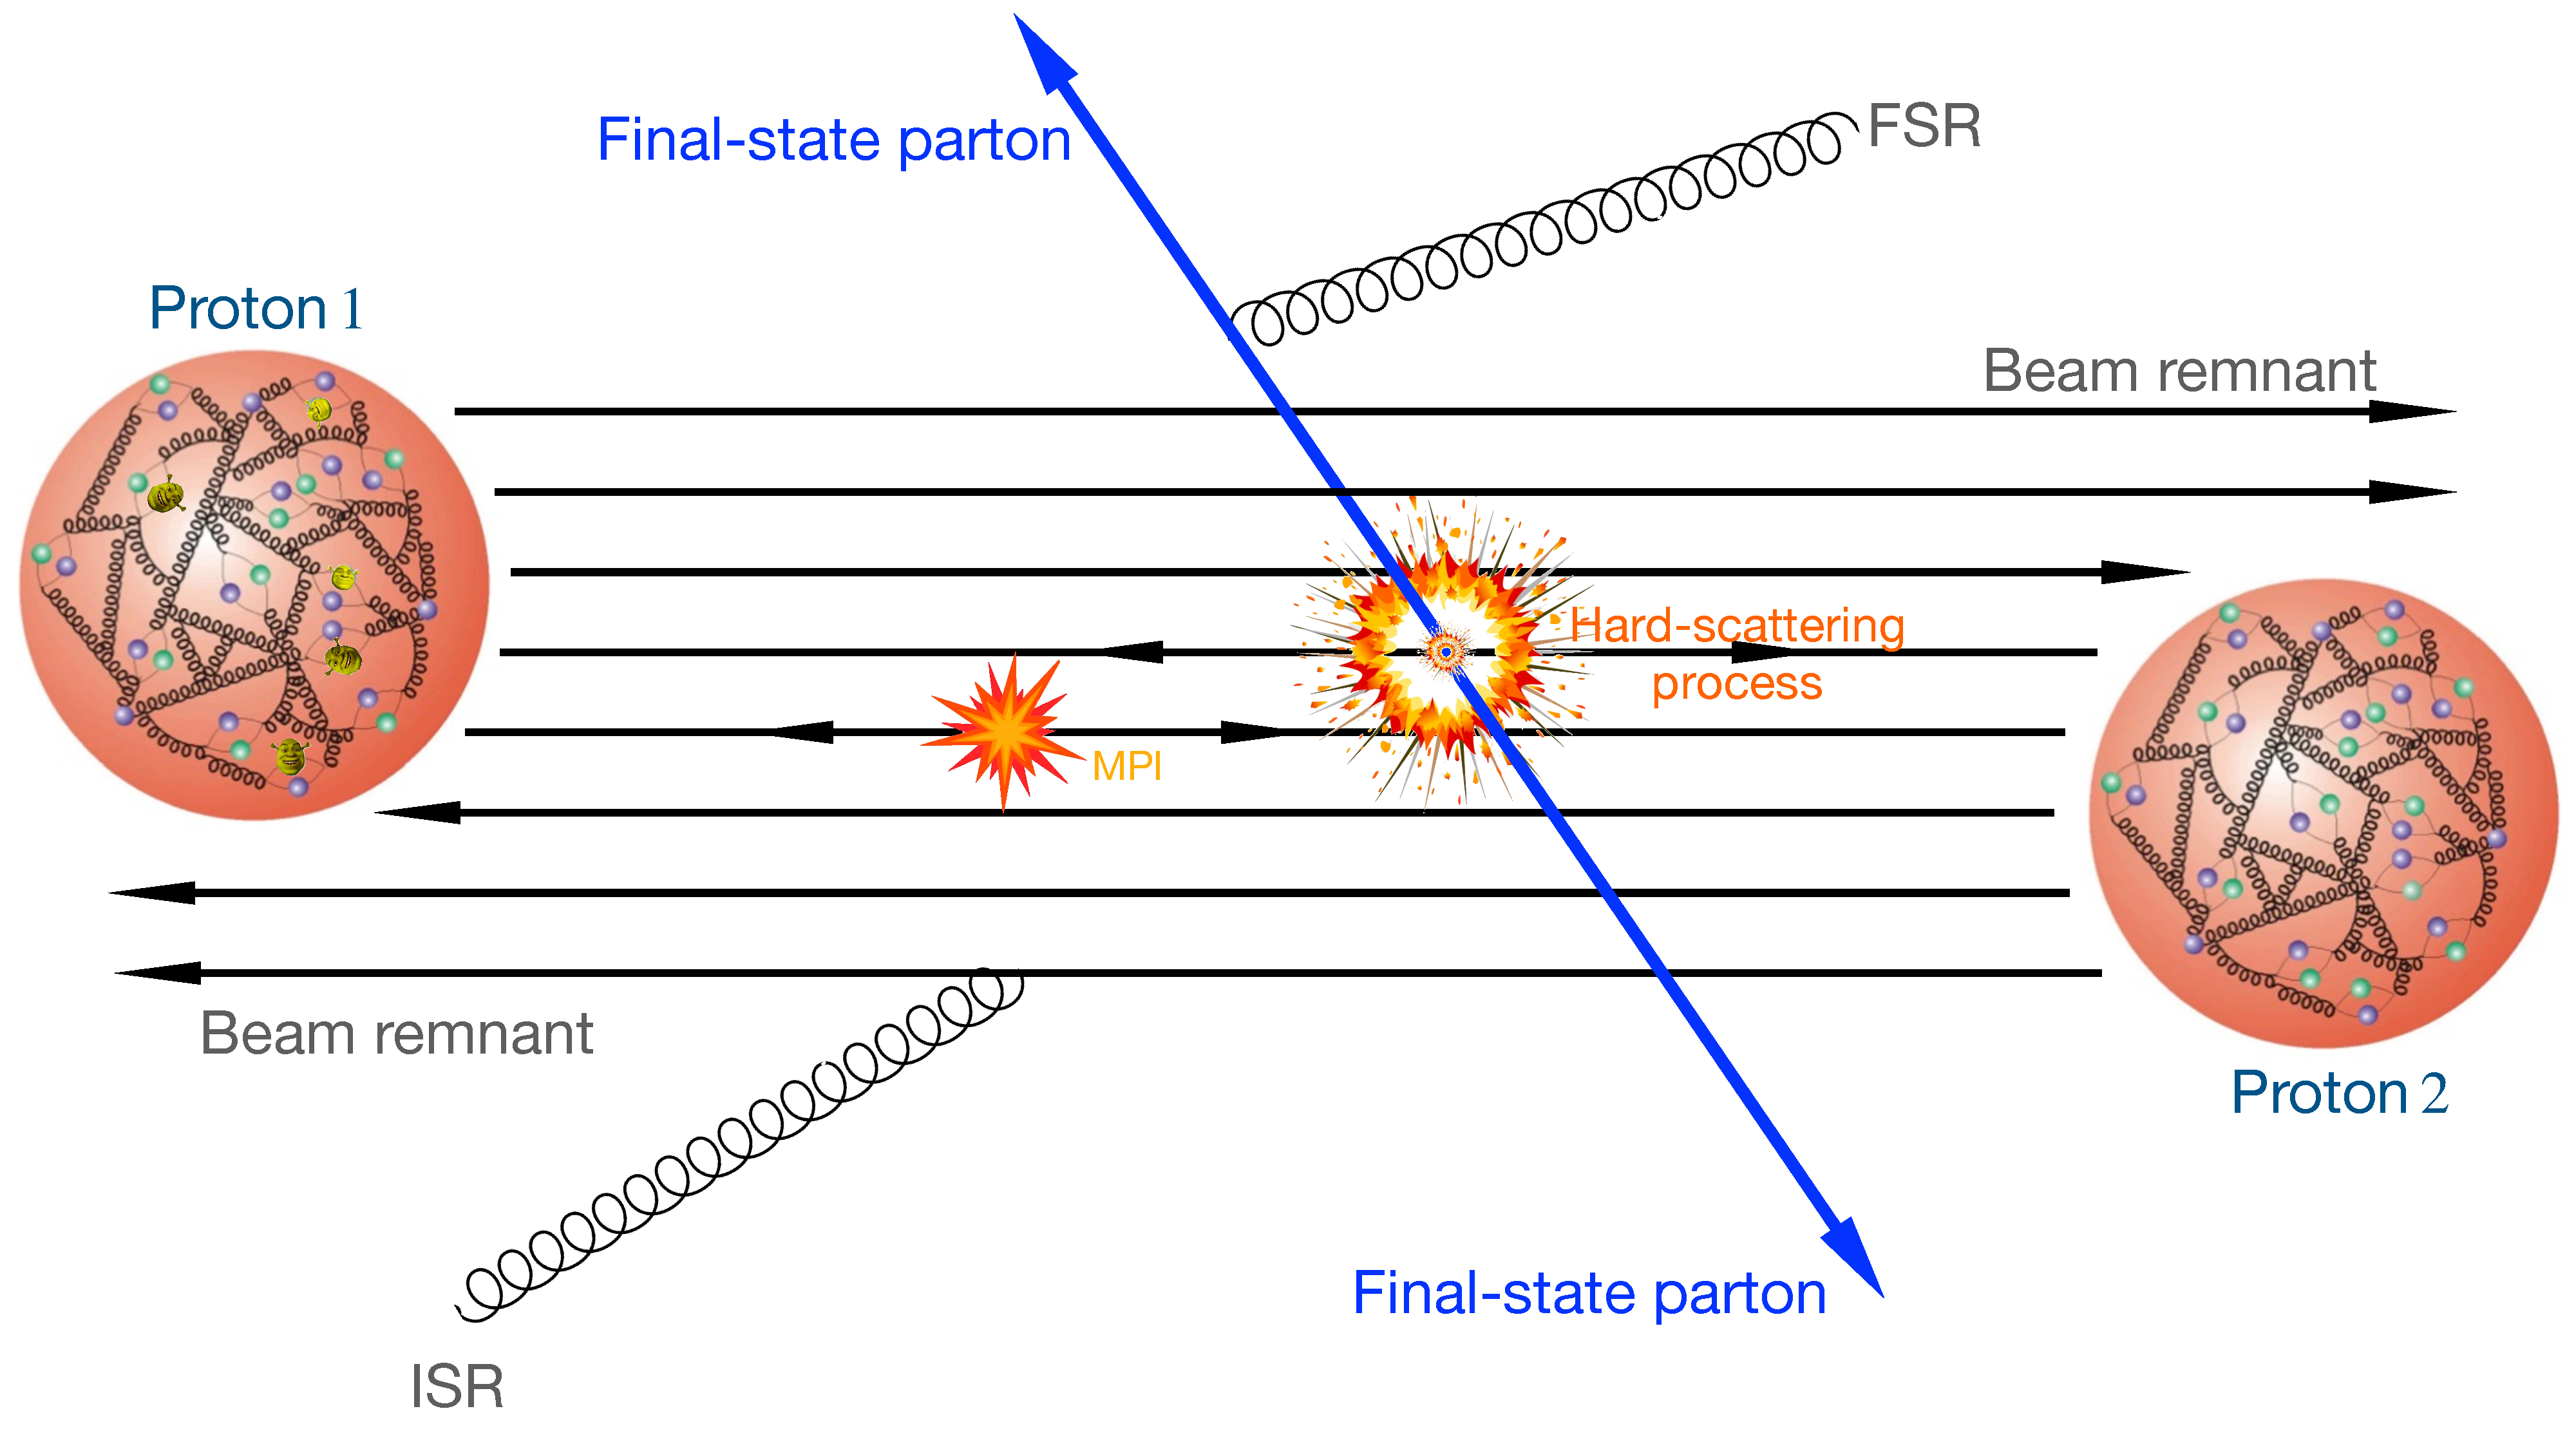
\includegraphics[width = 0.98\textwidth]{Chapter3/UnderlyingEvent_ByMe}
	\caption{Schematic representation of a $\Pproton\Pproton$ interaction.
	The collision consists of the hard-scattering interaction between two partons of the protons, 
	resulting in two final-state partons. 
	The UE includes additional components such as MPIs, ISR and FSR, 
	and particles originating from the break-up of the protons (i.e. beam--beam remnants). 
	It encompasses everything except the two outgoing hard-scattered particles.} 
	\label{fig:Chap2:UnderlyingEvent}
\end{figure}



%%%%%%%%%
%        pileup     %
%%%%%%%%%
%\subsection{Pile-up}
%\label{sec:Chap3.2:pileup}

%%%%%%%%%%%
%              Pile-up        %
%%%%%%%%%%%
\subsection{The pile-up effect} 
\label{sec:Chap2:LHC:pileup}

Pile-up is a challenging matter in terms of designing a detector and its DAQ system
as well as in the physics and performance analyses.
Because the LHC collides bunches of protons instead of single protons, multiple 
$\Pproton \Pproton$ interactions
occur at a single bunch-crossing\footnote{A bunch crossing is defined as the instance in which two 
collections of protons collide at the central region of the detector.}. Even with single protons this 
could happen since several partons of the two protons can intervene in the event.
This overlay can result in multiple collisions
at the same time and several interactions
with the same detector element, thereby generating overlapping signals which may be difficult
to differentiate. This is what is called pile-up.

As mentioned, the bunches are composed os $\sim10^{11}$~protons, but since the 
protons are so small compared to the bunch size, there are only around 
$30$ $\Pproton \Pproton$ collisions per bunch crossing with nominal beam at the LHC Run~2. 
This amount is also related to the crossing angle between the bunches ($\theta_{c}$).
The larger $\theta_{c}$, the smaller is the area of overlap between the bunches and, hence,
the smaller is the possibility of a collision.
The mean number of interactions (<$\mu$>)
per bunch crossing is presented in Figure~\ref{fig:Chap2:LHC:PileUp_15-18} for the three
runs of the LHC. Note that for each run, since the instantaneous luminosity is increased, 
the pile-up is higher than for the previous run. %This increase does not only take place from
%one run to the next but also with time within a single run. 
%(as it is later presented in Section~\ref{sec:ChaptH:Data_and_MC:Data}).
%The mean number of interactions per bunch crossing 
The <$\mu$>
corresponds to the mean of the Poisson distribution of the number of interactions per crossing 
calculated for each bunch. It is calculated from the instantaneous luminosity produced by a single 
pair of colliding bunches ($\mathcal{L}_{\text{bunch}}$),
the inelastic cross-section 
and revolution frequency as 
<$\mu$>$\,= \mathcal{L}_{\text{bunch}} \times \sigma_{\text{inel}} / f$~\cite{ATLAS:2022hro}. %where  is the 
%instantaneous luminosity per bunch, which is described by equation~\ref{eq:Chap2:LumiInst}.
%The term $\sigma_{inel} = 80$~mb is the inelastic cross-section of $\Pproton \Pproton$ collisions at $13$~TeV
%and $f_{r}=11.245$~kHz is the LHC revolution frequency.

%The modelling of the pile-up is described in detail in Section~\ref{chap:DataAndMC:pileup}.

\begin{figure}
	\centering
 	 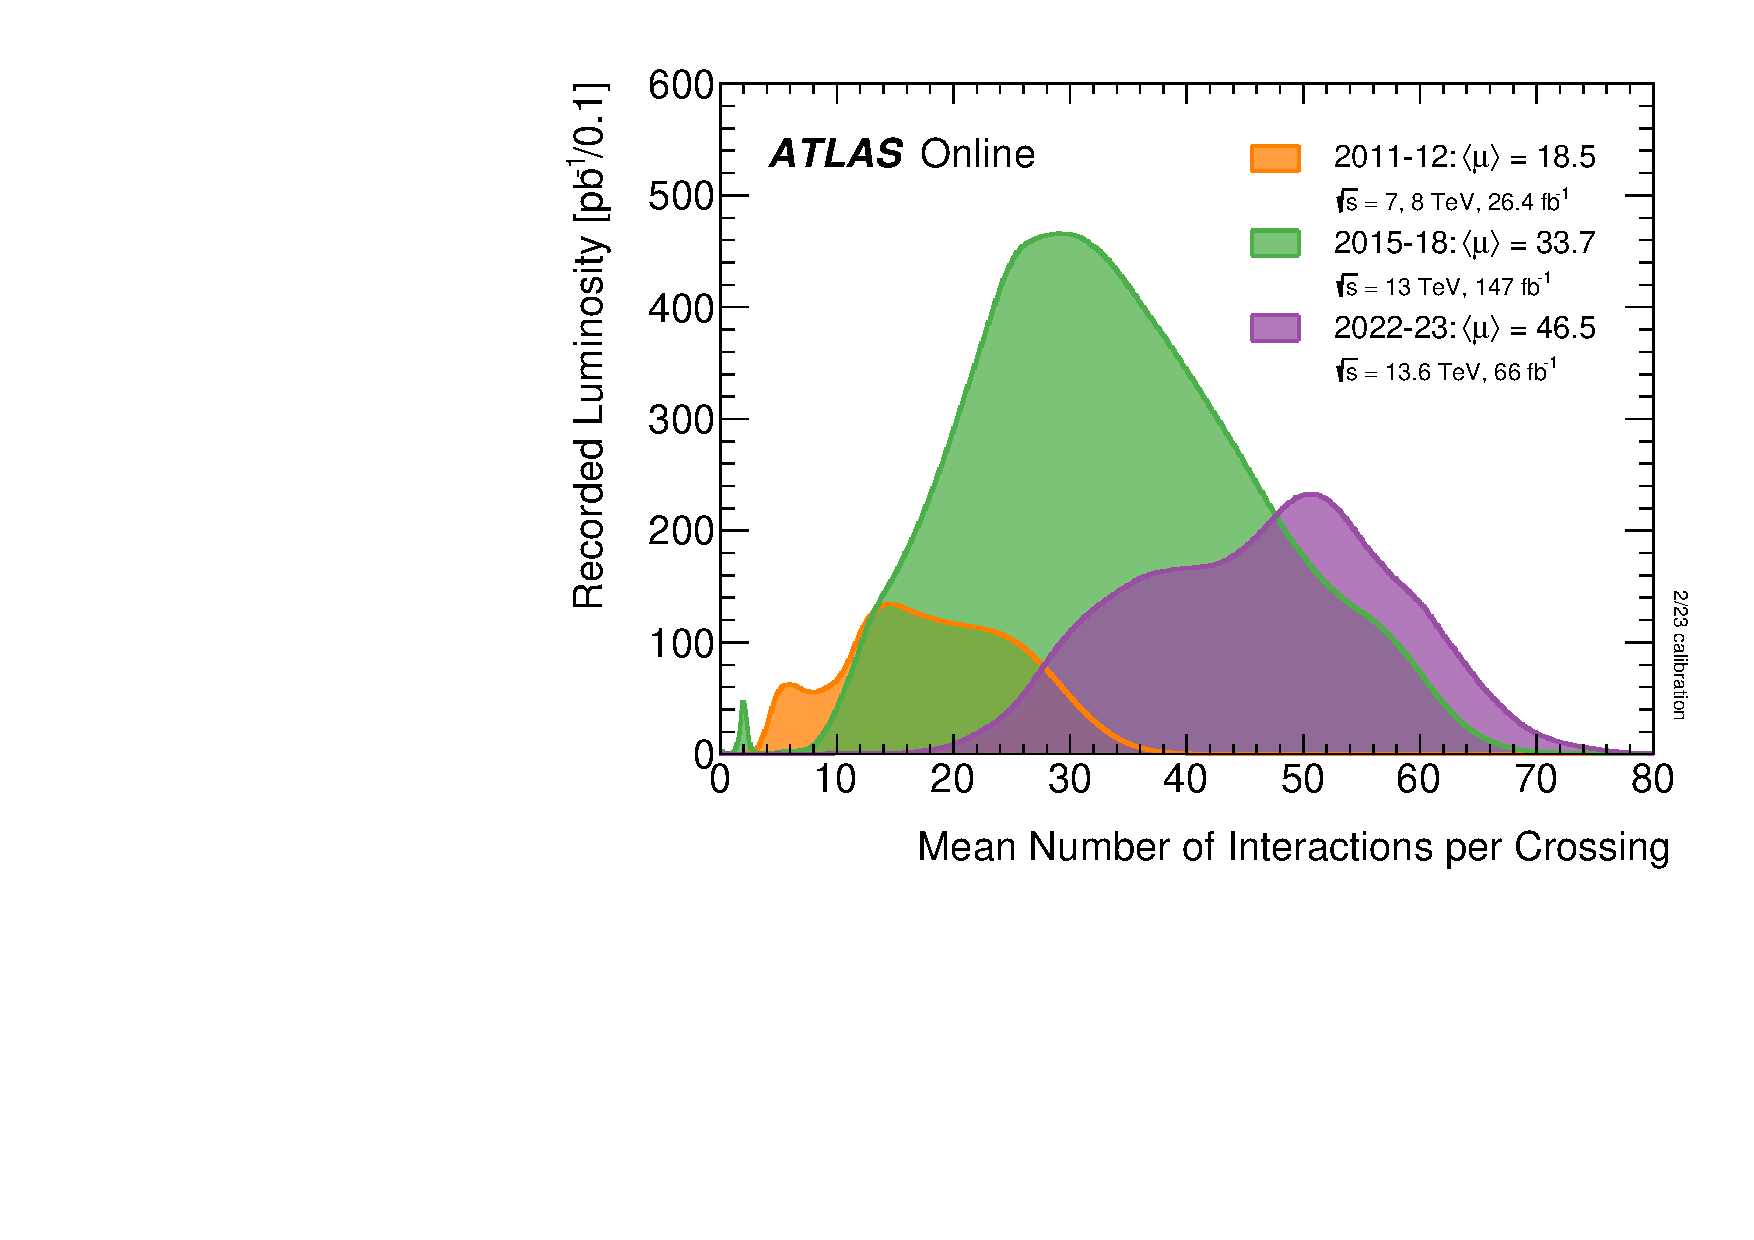
\includegraphics[width = 0.85\textwidth]{Chapter2/Pile-up_Runs_1234.pdf}
	 \caption{Luminosity-weighted distribution of the mean number of interactions 
	 per crossing, <$\mu$>, in $\Pproton \Pproton$ collisions at $\CM=7$ and $8\,\text{TeV}$ during Run~1 (orange),
	 $\CM=13$~TeV during Run~2 (green), and $\CM=13.6$~TeV at Run~3.
	 All physics-data recorded by the ATLAS detector during stable beams in these years are shown (until July 2023)~\cite{ATL-DAPR-PUB-2023-001}.}
	 %, Run~2 and Run~3, with $\Pproton \Pproton$ collisions data during stable beams at $\CM=13$~TeV.}
	\label{fig:Chap2:LHC:PileUp_15-18}
\end{figure}

%Luminosity levelling is generally applied to reduce the number of collisions per bunch crossing 
%in the experiments when the instantaneous luminosity is too high. In 2017, when the 8b4e and 
%the 8b4e-BCS beams were used the peak luminosity exceeded the pile-up limit of ATLAS and CMS~\cite{steerenberg2019operation}

%According to equation~\ref{eq:Chap2:LumiInst}, there are three possible ways of 
%increasing the luminosity:

%\pablo{Work in progress}




%\cite{ATLAS:2010arf}




%%%%%%%%%%%
%        Luminosity     %
%%%%%%%%%%%
\subsection{Luminosity}
\label{sec:Chap1:LHC:Cross-Luminosity}
%\paragraph{Luminosity}\mbox{}\\
Luminosity is a measure of the number of collisions that take place in a time frame.
It plays a pivotal role in determining the rate at which particle interactions occur, 
thus influencing the experimental data obtained.
Besides the centre-of-mass energy, the luminosity is the most relevant parameter to characterise
a collider-based experiment, and it is especially 
important in searches for processes with small production cross-section
(known as rare processes).
It measures the ability of the particle accelerator to produce enough events of a desired type.

The instantaneous luminosity, $\lumi(t)$, is the ratio of events produced in a 
certain period of time for a given cross-section $\sigma$:
\begin{equation*}
\lumi = \frac{1}{\sigma}\frac{dN}{dt} = \frac{1}{\sigma} R \, ,
\end{equation*}
where $N$ is the number of the events and $t$ the time. The symbol $R=\frac{dN}{dt}$ is 
known as event rate. It can be understood as the number of particle collisions per 
unit of area (typically expressed in cm$^2$) and per second, therefore it is 
measured in \lumiunits~\cite{Herr:941318}.  Alternatively, the luminosity
can also be expressed in barns\footnote{A barn is a metric unit of area following the equivalence
$1\text{b}=10^{-28}\text{m}^2$.}.
 
% The luminosity is proportional to the number of bunches per beam ($n$), the revolution frequency ($f$) and the number 
%of particles in each bunch ($N_1$ and $N_2$), and inversely proportional to the beam cross-section ($A$)
%\begin{equation}
%\lumi = \frac{nfN_{1}N_{2}}{A}
%\end{equation}

The instantaneous luminosity is proportional to the number of protons  
in each of the bunches that collide head-on ($n_1$ and $n_2$), the revolution frequency ($f$) with 
which the bunches are crossing, and the number of proton bunches in the machine ($n_b$).
The $\lumi$ is inversely proportional to the effective transverse area of the beams
in which the collision takes place ($4 \pi\sigma_{x} \sigma_{y}$):
\begin{equation}\label{eq:Chap2:LumiInst}
\lumi = f \cdot \frac{n_{1} n_{2} n_{b}}{4 \pi\sigma_{x} \sigma_{y}}\cdot F(\theta_{c},\sigma_{x},\sigma_{z})\, ,
\end{equation}
where $F(\theta_{c},\sigma_{x},\sigma_{z})$ is a factor accounting for the luminosity reduction due to the beam-crossing angle ($\theta_c$).
At the LHC, assuming that the particles travel at the speed of light, for its $27$~km long, 
the bunch-crossing frequency is $f = 11.2455$~kHz. 
The maximum number of proton bunches in the machine is\footnote{The theoretical maximum of 3564 bunches cannot 
be reached due to space needed between bunch trains and for the beam dump kicker magnets.} $n_b$ = 2808
(see Table~\ref{tab:Chap2:LHC:Parameters}). 
 In each bunch, there are $n_1 \approx n_2 \approx 1.2 \times 10^{11}$ particles at the LHC Run~2. 
 Finally, characterising the optics of the collision at the IP, the root mean square transverse beam width in the horizontal and vertical directions are $\sigma_{x} \approx \sigma_{y} \approx 12, ... , 50$~\textmu m. Equation~\ref{eq:Chap2:LumiInst} assumes that the particles in the beam follow a Gaussian distribution.
According to equation~\ref{eq:Chap2:LumiInst} the instantaneous luminosity only depends on the machine and its beam parameters~\cite{ATLAS:2016fhk}. %Hoecker:2016vvy,
The instantaneous luminosity for %the LEP collider was $\lumi_{\text{LEP}}=1.0\times10^{32}$\lumiunits  and 
the LHC is designed to achieve $\lumi_{\text{LHC}_{pp}}=2.1\times10^{34}$\lumiunits 
in $\Pproton\Pproton$ collisions and $\lumi_{\text{LHC}_{\text{PbPb}}}=6.1\times10^{27}$\lumiunits for heavy ion collisions.
     

The integrated luminosity ($L$) over time is given by 
\begin{equation*}
	 L = \int \lumi \, dt \, ,
\end{equation*}
 and it is used to determine the number of events, $N$, that have taken place during 
 that time within the detector, i.e. $N = \sigma \times L$. 
 Therefore, the number of observed events is:
 \begin{equation*}
	N^{\text{obs}}_{\text{events}} = \sigma_{\text{process}} \times \text{efficiency} \times L \, ,
 \end{equation*}
where the efficiency of the detection has to be optimised experimentally, the $L$ is delivered
by the LHC and the cross-section of the 
process ($\sigma_{\text{process}}$) is given by nature. The efficiency accounts for the 
geometrical acceptance of the detector, trigger efficiencies, and the reconstruction and
identification of physical objects. 

Several factors can limit the maximum luminosity that can be achieved at the LHC~\cite{Herr:941318} 
such as the beam--beam effect, crossing angle, beam offset or the hourglass effect. 
On the other hand, there are diverse strategies to maximise the luminosity delivered 
by a machine (e.g. maximise the total beam current or %~\cite{Hoecker:2016vvy}
compensate reduction factor).

\begin{comment}
\begin{itemize}
	\item \textbf{Beam--beam effect}: The bunches of two beams or the particles in the same bunch can interact electromagnetically, this leads to distortions from the orbit and results in an increase of the emittance, $\epsilon$.
	\item \textbf{Crossing angle}: Often used to avoid unwanted collisions in machines with many bunches, due to the crossing angle $\theta_c$, 
				the luminosity is reduced by a factor $F(\theta_{c},\sigma_{x},\sigma_{z}) = \sqrt{1+(\theta_{c}\sigma_{z}/2\sigma{x})^2}$.
	\item \textbf{Beam offset}: Originated from the beam-beam effects or misalignments in the quadrupole magnets, the beams can collide with 
				small transverse offset. Such beams' offsets induce a loss of $\lumi$ at the IP.
	\item \textbf{Hourglass effect}: Appears when beams collide in a point away from the IP. 
\end{itemize}

\begin{itemize}
	\item \textbf{Maximise the total beam current}: Improvements in beam collimation, cryogenics vacuum and background protection could extend the limit on the maximum beam current. 
	\item \textbf{Compensate reduction factor}: The hourglass effect may be reduced by shorter bunches at the expense of a higher longitudinal pileup density (see Section~\ref{sec:Chap2:LHC:pileup}).
\end{itemize}
\end{comment}




%%%%%%%%%%%
%               Data          %
%%%%%%%%%%%
\section{Recording data with the ATLAS detector}
\label{sec:Chap3.1:Data}
%\begin{itemize}
%	\item How is data collected in ATLAS? DAQ
%	\item Pileup (differentiate LHC pileup from ATLAS pileup during Run~2)
%	\item What are triggers
%\end{itemize}
%\pablo{Revisar título de esta sección}

The ATLAS experiment produces an enormous amount of 
data through high-energy $\Pproton \Pproton$ collisions. To
interpret of this vast volume of information, a well-defined data 
model is crucial. %In this section, we explore the ATLAS data 
%model and discuss key concepts such as luminosity and pile-up.

The ATLAS data model serves as the foundation for organising 
and managing the recorded data. It provides a standardised and structured framework 
that allows to access and analyse data effectively. %This 
%data format is briefly discussed in Section~\ref{sec:Chap3.1:Data:Model}.
In Figure~\ref{fig:Chap3:SimVsReal} the ATLAS data model is presented
by comparing, at each level, the real-detector data with the simulated event data.

 \begin{figure}
    \centering
    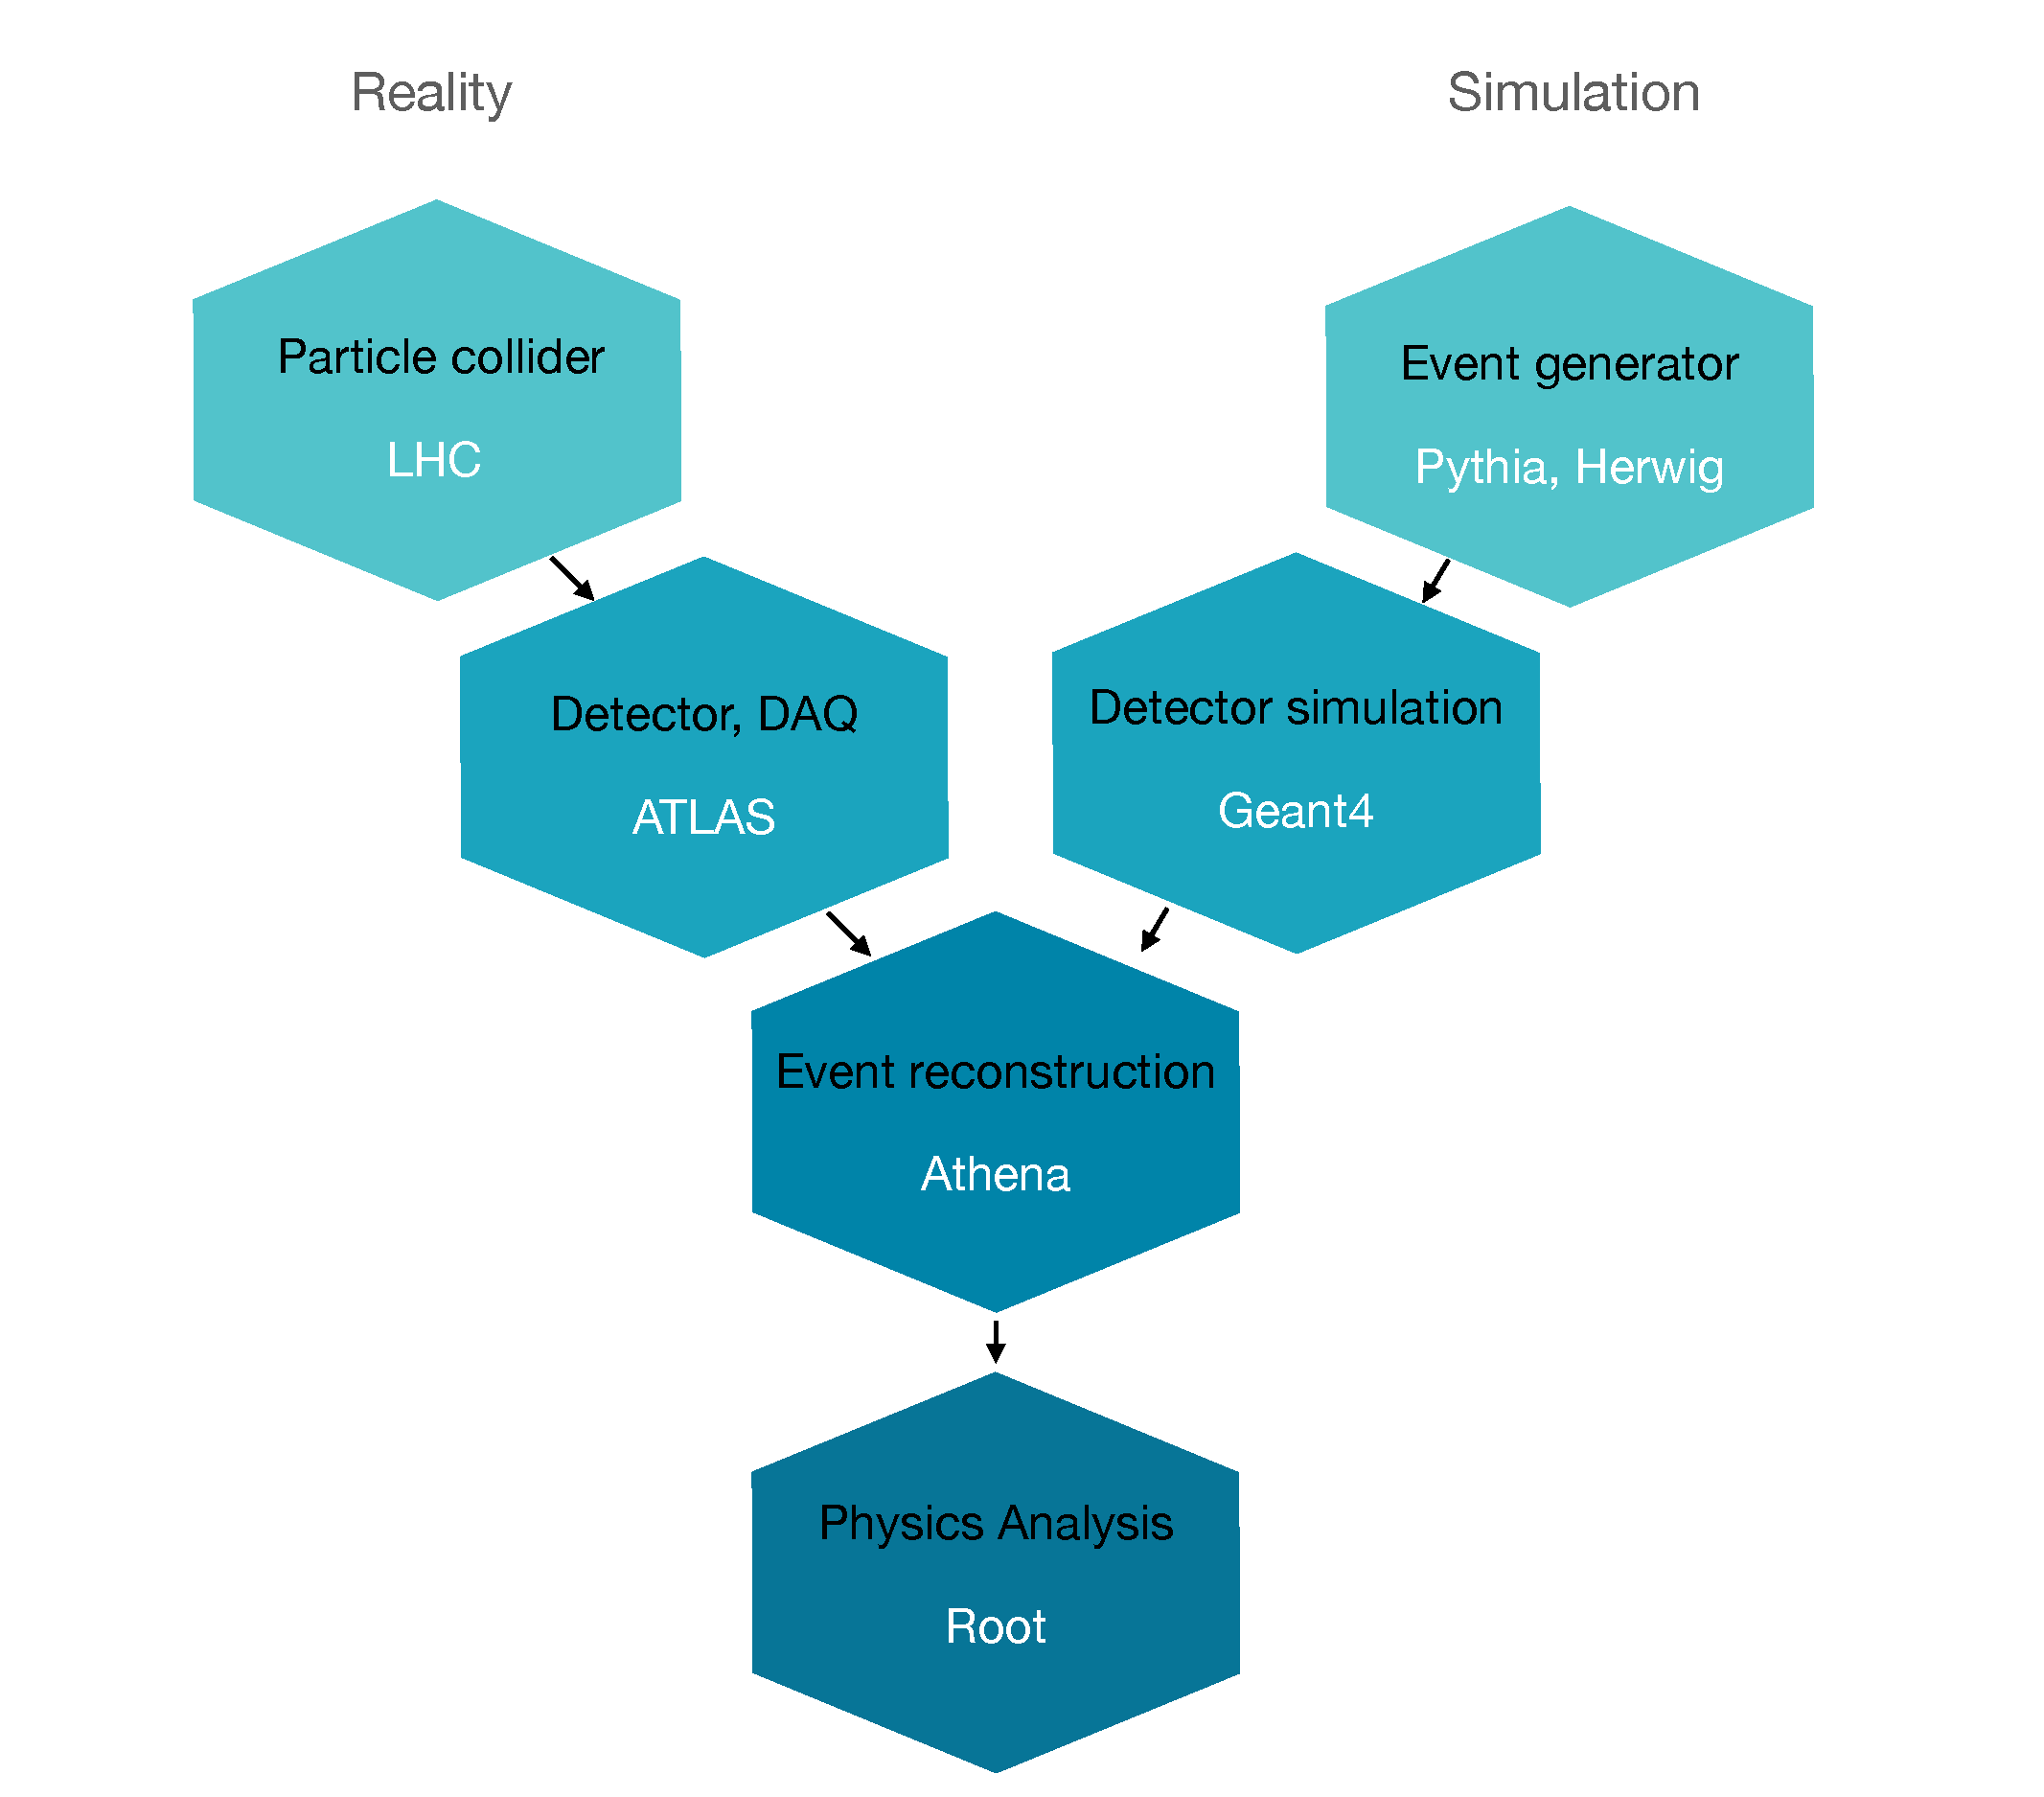
\includegraphics[width = \textwidth]{Chapter3/SimulationVSRealityChain.pdf}
    \caption{Comparison of the paths followed by data recorded by the ATLAS detector and the simulated samples.
    At each step, the format of the simulated data is the same as the recorded data.}
    \label{fig:Chap3:SimVsReal}
\end{figure}


%As already mentioned, one of the fundamental concepts in particle physics is luminosity, 
%which quantifies the number of collisions occurring per unit time. 
%It is a measure of the intensity of the particle beams and determines 
%the overall collision rate. The cumulative luminosity plays a crucial role in determining 
%the statistical significance of measurements and is described in Section 
%\ref{sec:Chap3.1:Data:DeliveredLuminosity}.

%Another concept closely related to luminosity is pile-up, which is discussed
%in Section~\ref{sec:Chap2:LHC:pileup}. Pile-up refers to the presence 
%of additional proton--proton collisions within the same bunch crossing. 
%These additional collisions produce extra particles and contribute to 
%the overall background in the detector. Effectively managing and understanding 
%pile-up is crucial for distinguishing the signals of interest from the 
%background and ensuring accurate measurements.




\begin{comment}
%
% ATLAS Analysis model
%
\subsection{ATLAS data model}
\label{sec:Chap3.1:Data:Model}
ATLAS implements a standardised data format for reconstruction and analysis, 
supported by a data reduction framework, to generate prefiltered samples\footnote{A 
sample is a collection of events, a dataset.} for 
physics groups in a production environment. This framework facilitates the reuse 
of tools by physics groups at local levels.~\cite{Buckley:2015tjh} %\cite{Brun:1997pa}

The primary data format used in ATLAS is ROOT~\cite{Brun:1997pa}, which connects the reconstructed 
objects to the analysis stage. For Run~2, a novel data model was introduced, combining the advantages 
of rapid retrieval of event groups and optimised storage utilisation. In many physics analyses, intermediate-sized
 data products play a pivotal role in the early stages of the analysis workflow. These data formats are 
 typically derived directly from the preserved output of the reconstruction process, referred to as 
 Analysis Object Data (AOD) within ATLAS. Such formats exhibit common characteristics, including:
 
 \begin{enumerate}
 	\item Central Production: These data products are generated centrally for both experimental data and simulated events. 
		Their size is typically ranging from a hundredth to a thousandth of the original input data size.

 	\item Analysis Focus: AODs are specifically designed to cater to the requirements 
		of a particular analysis or a group of related analyses that share similar characteristics 
		(for instance, having the same final state objects).

 	\item Calibration and Selection: During their creation, AODs incorporate essential calibrations and 
		object selections. These calibration schemes are often shared among different physics 
		groups to ensure consistency.

  	\item Comprehensive Information: AODs encompass all the necessary information to 
		facilitate essential operations on reconstructed objects, such as smearing, scaling, 
		selection, and calibration. They also incorporate the systematic uncertainties associated 
		with these operations, collectively known as combined performance operations in ATLAS.

 	\item Reproduction and Accessibility: These intermediate data products are typically 
		reproduced 10-12 times per year. However, they are frequently accessed by 
		analysis teams, with multiple reads per week, to perform subsequent analyses 
		and investigations.
 \end{enumerate}
 
 By adhering to these characteristics, the AODs within ATLAS streamline the 
 analysis process, enable efficient data handling, and provide a comprehensive and robust foundation 
 for performing various performance operations and systematic uncertainty evaluations on 
 reconstructed objects.
 
ATLAS employs various data reduction operations to streamline the analysis process.
These reduction operations are categorised as follows:
\begin{itemize}
	\item Skimming: This operation involves the removal of entire events based on specific 
		criteria related to the characteristics of the event. Events that do not meet the defined 
		criteria are excluded from further analysis.
	
	\item Slimming: Slimming involves the uniform removal of variables\footnote{A 
		variable is a property of the event or of one of its constituents (‘feature’ in
		machine learning)} within a particular type of 
		object across all objects and events. The same set of variables is eliminated for every 
		instance of the object, ensuring consistency in the data reduction process.
	
	\item Thinning: Thinning focuses on the removal of individual objects within an event based on 
		predetermined criteria associated with the properties of the object. For example, objects
		failing to satisfy certain kinematic requirements may be discarded.

	\item Augmentation: Augmentation entails the addition of supplementary information during the 
		data reduction operation to enhance the analysis capabilities. This augmentation is typically
		done in two ways:
		\begin{itemize}
			\item Adding new reconstructed object containers. For instance, jets made with a modified algorithm.
			\item Decorating existing objects with extra variables. For example, the results of object selection by 
				combined performance tools such as ``this is a good muon''.
		\end{itemize}
\end{itemize}
% Good source: https://indico.cern.ch/event/472469/contributions/1982677/attachments/1220934/1785823/intro_slides.pdf

The flow of the data model, as depicted in Figure~\ref{fig:Chap3:Analysis_data_model_ATLAS}, 
involves the use of the derivation framework for data reduction. Within this framework, intermediate 
data products are generated by selectively discarding or incorporating information to the reconstruction output 
(i.e. AOD), while preserving the underlying structure and event data model of the original AOD. 
The analysis framework serves as the final component of the model, providing physicists with 
the means to access the derived data products, apply various combined performance tools, and 
generate the ultimate small NTuples\footnote{Ntuple is a data structure used to store information about each event.}. 
These NTuples serve as the basis for creating plots and 
conducting subsequent statistical analyses. In other words, the AODs are too large to analyse directly 
and hence, the derivation framework reduces them to create the various DAODs (also known as derivations). 
DAODs are still made of xAOD objects, but are much smaller. 
This data model is embedded within
the ATLAS software framework, Athena\footnote{Athena is the framework used for all pre-analysis data processing; it can also be
used for physics analysis.}.


\begin{figure}
 	 \centering
 	  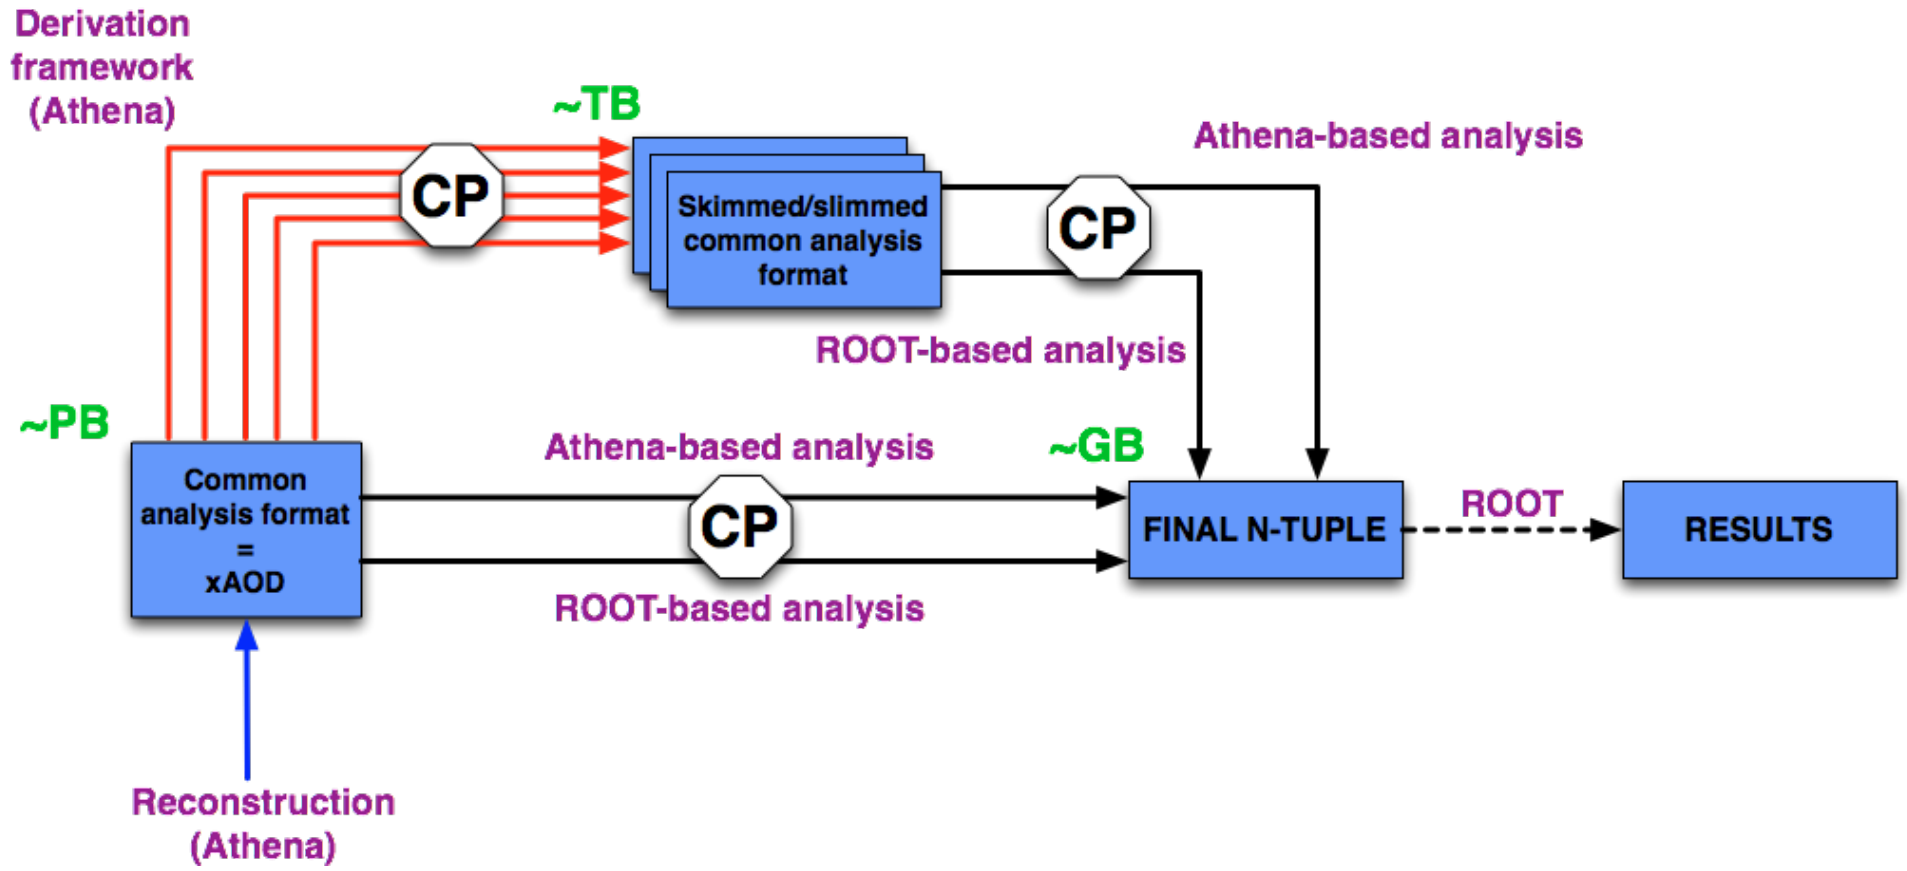
\includegraphics[width = 0.8\textwidth]{Chapter3/ATLAS_Run_2_Analysis_model}
	  \caption{Analysis model employed in ATLAS during Run~2. The scheme illustrates the transformation 
	  of the reconstruction output, known as AOD, through the derivation framework. This process results in 
	  the generation of multiple streams of Derived Analysis Object Data (DAOD). The original AOD and the 
	  derived DAOD possess compatible data models, allowing the analysis software to seamlessly use 
	  either format as input~\cite{Brun:1997pa}. In this Figure CP stands for Combined Performance groups}
	\label{fig:Chap3:Analysis_data_model_ATLAS}
\end{figure}
\end{comment}



%
% Lumi
%

%%%%%%%
%. Delivered luminosity
%%%%%%%
\subsection{Cumulative luminosity}
\label{sec:Chap3.1:Data:DeliveredLuminosity}
In Section~\ref{sec:Chap1:LHC:Cross-Luminosity} a description of 
instantaneous and integrated luminosity is given. Here the cumulative-luminosity
results for the ATLAS detector during Run~2 are presented for each year. 
The importance of these details lies in the fact that this is the dataset
used for the research presented in this thesis.
The cumulative luminosity plays a crucial role in determining 
the statistical significance of measurements 

The cumulative luminosity delivered by the LHC to the ATLAS detector is 
shown in Figure~\ref{fig:Chap2:intlumivsyear} for every year of LHC operation. 
In Figure~\ref{fig:Chap2:intlumivstimeRun2DQall}, the total Run~2 cumulative luminosity is presented differentiating between the delivered
and recorded luminosity and showing that almost all delivered events are considered to have good data quality. 
Note that the luminosity delivered by the LHC machine is not the same as the
one registered by the ATLAS detector, although these numbers are very close.
The delivered corresponds to the luminosity delivered by the LHC machine 
to the detector and, ideally, should be fully recorded. But in some
cases, the ATLAS detector is unable to take data either because 
one or more subdetectors are temporally unavailable or because its
DAQ chain is busy (see Section~\ref{sec:Chap2:Trigger_and_DAQ}).
% The delivered luminosity accounts for the luminosity given from the start of stable beams until the LHC control 
% requests to put the ATLAS detector in a safe standby 
% mode to allow a beam dump or beam studies. The recorded luminosity reflects the DAQ inefficiency, as well as the inefficiency of the 
% so‐called ``warm start''\footnote{When the stable beam flag is raised, the tracking 
% detectors undergo a ramp of the high-voltage and, for the 
% pixel system, turning on the preamplifiers.}.
The data quality algorithms check  the operation of the detectors and the performance of the physical 
object reconstructors to decide which data should be accepted.
The \texttt{All Good Data Quality} criteria is used and it requires all reconstructed physics objects to be of good data quality~\cite{ATLAS:2019fst}.  For the entire Run~2 dataset, 95.6\% of events are labelled as good for physics
and are included in the \texttt{Good Run Lists}  (GRLs).

\begin{figure}[h]
 	 \centering
 	  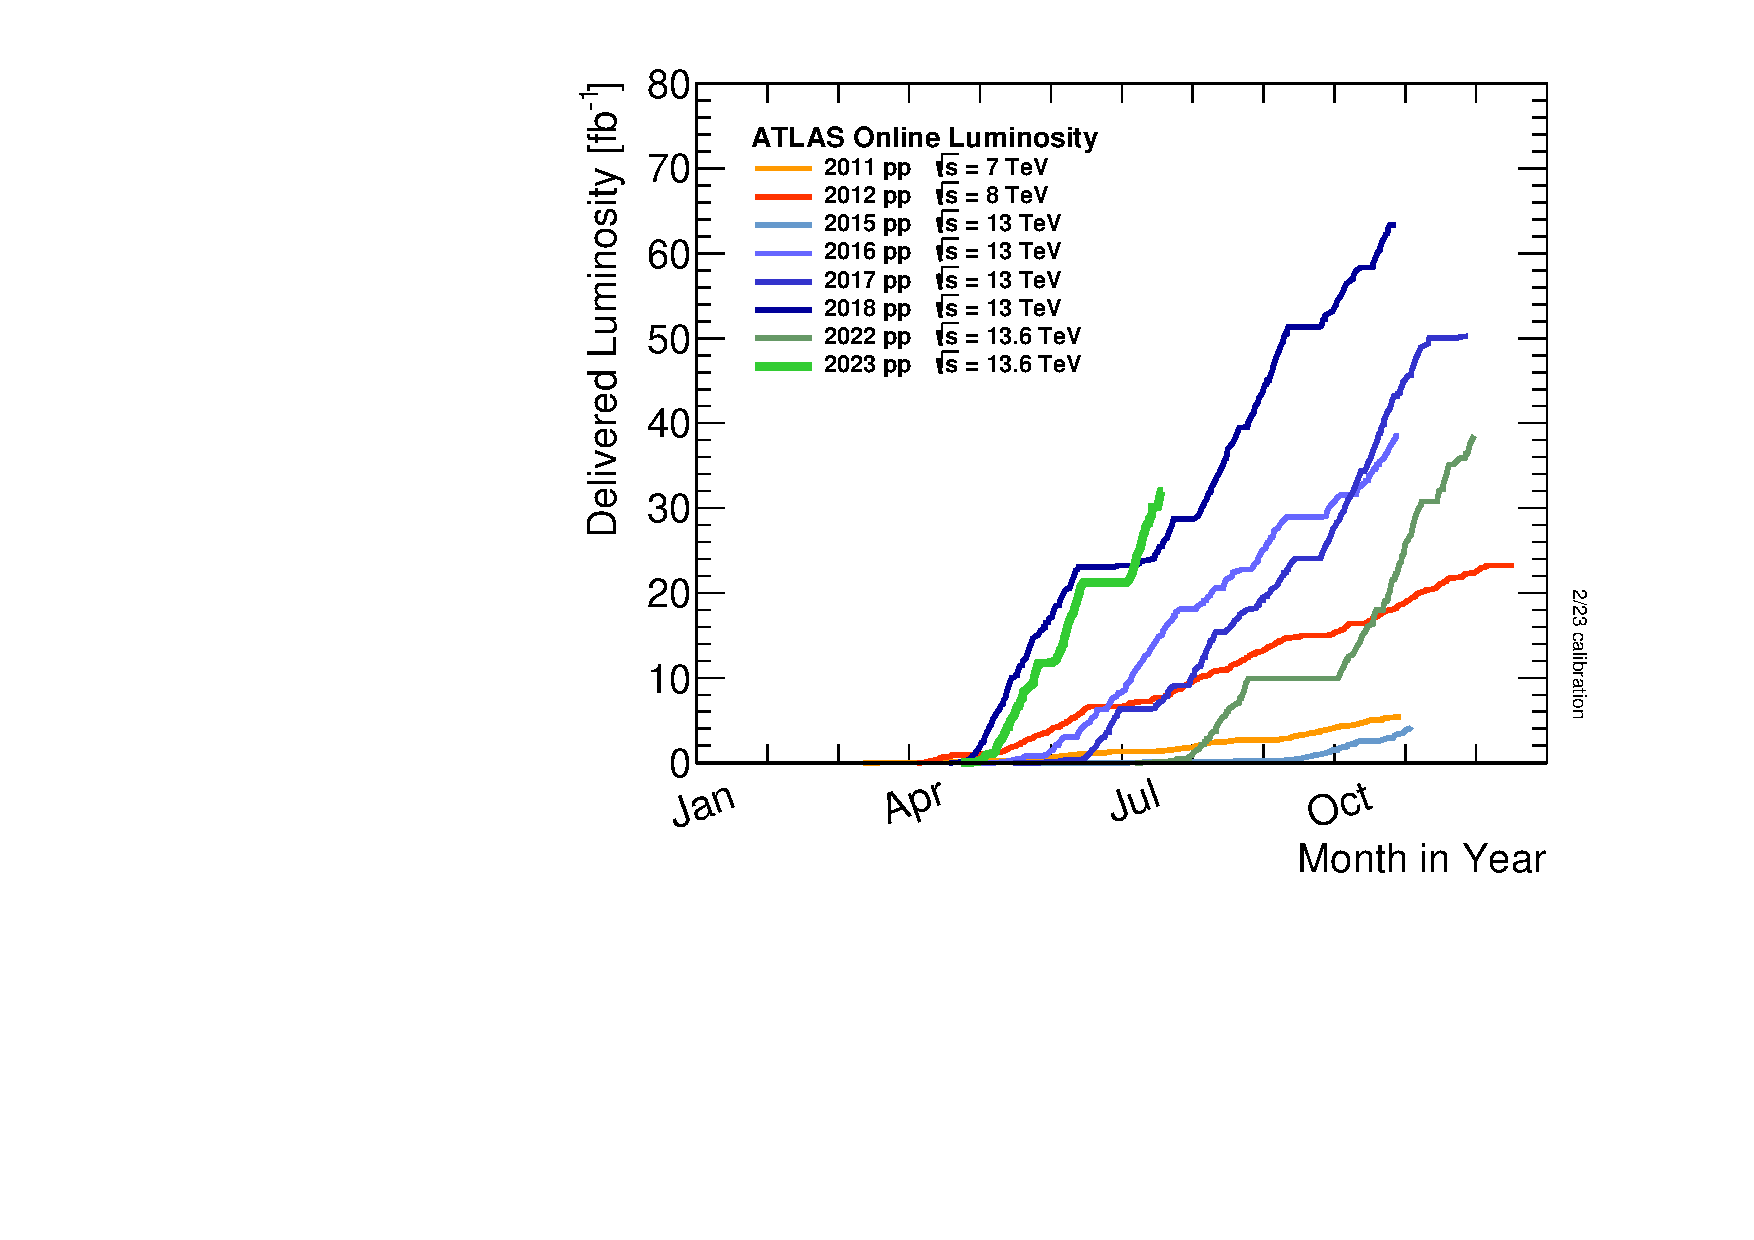
\includegraphics[width = 0.9\textwidth]{Chapter2/intlumivsyear_extended}
	  \caption{Cumulative luminosity versus day delivered to the ATLAS detector by the LHC during stable 
	  beams and for high energy $\Pproton\Pproton$ collisions for Run~1, Run~2~\cite{ATLAS:2019fst, ATLAS:2022hro} 
	  and Run~3~\cite{ATL-DAPR-PUB-2023-001}.}
	\label{fig:Chap2:intlumivsyear}
\end{figure}

%\begin{table}[h]
%\centering
%\resizebox{\textwidth}{!}{
%\begin{tabular}{lllll}
%\toprule
%Year                                     							& 2015				& 2016 		& 2017 		& 2018 	\\ \midrule
%Peak $\mathcal{L}(t)$ ($\times 10^{33}$~\lumiunits)	& 5					& 13			& 16			& 19 		\\
%Total delivered $L$ (fb$^{-1}$) 			& 4.0					& 38.5 		& 50.2 		& 63.4 \\
%$L$ registered by ATLAS ($\text{pb}^{-1}$)	&$3244.54\pm1.13\%$ & $33402.2\pm0.89\%$ & $44630.6\pm1.13\%$ & $58791.6\pm1.10\%$  \\
%\bottomrule
%\end{tabular}}
%\caption{Peak luminosity, integrated luminosity delivered by the LHC and 
%cumulative luminosity collected by the ATLAS detector at $\CM = 13$~TeV during Run~2 per year~\cite{ATLAS:CONF:2019:021}. 
%The uncertainties are measured with the LUCID-2 detector~\cite{ATLAS:2022hro, Avoni:2018iuv}.} 
%\label{tab:Chap2:LHC:LumiRun2}
%\end{table}

\begin{figure}[h]
 	 \centering
 	  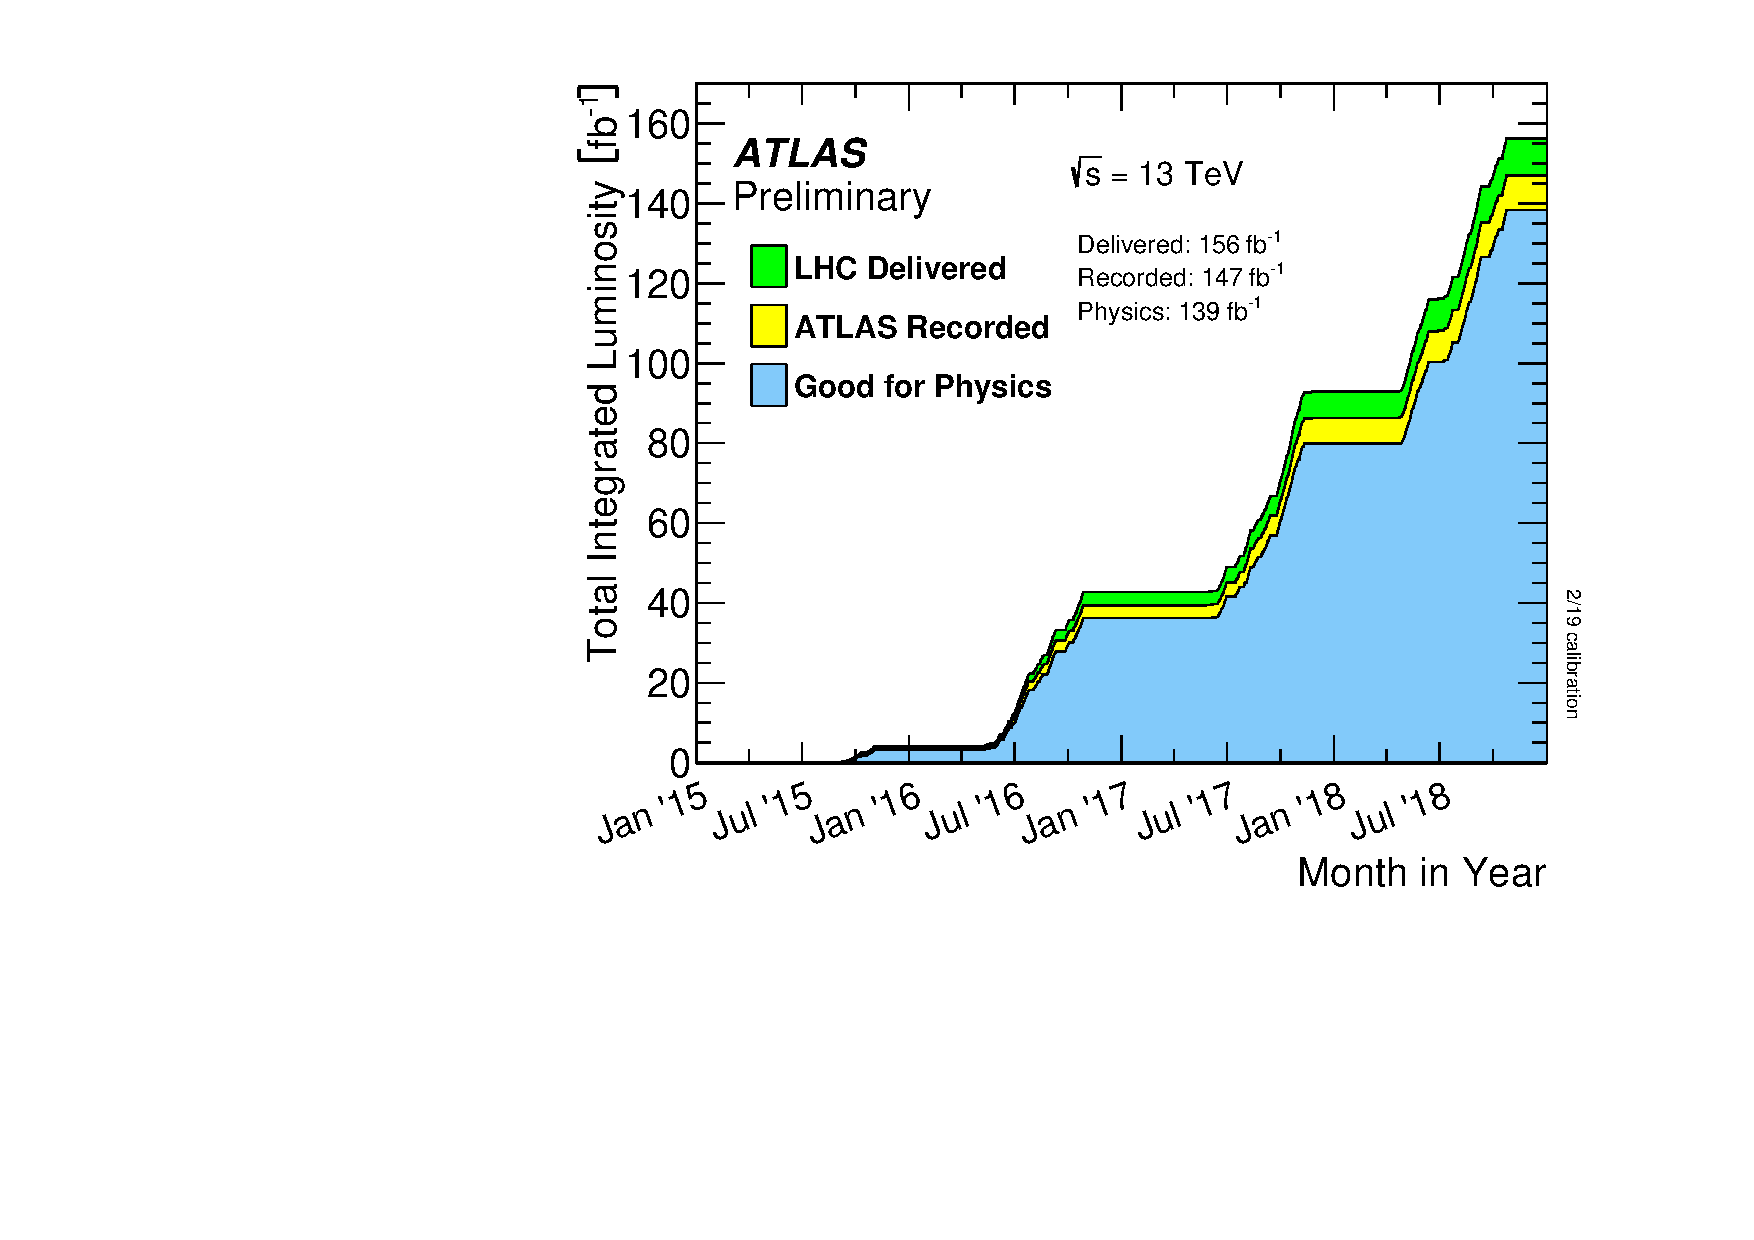
\includegraphics[width = 0.9\textwidth]{Chapter2/intlumivstimeRun2DQall}
	  \caption{Total cumulative luminosity versus time delivered to ATLAS (green), 
	  recorded by the ATLAS detector (yellow) and passing the good-quality-data 
	  requirements for ATLAS physics analyses (blue) during stable beams for 
	  $\Pproton\Pproton$ collisions at $\CM = 13$ TeV during Run~2~\cite{ATLAS:2019fst}.}
	\label{fig:Chap2:intlumivstimeRun2DQall}
\end{figure}
%http://www.personal.soton.ac.uk/ab1u06/teaching/phys3002/course/13_accelerators_a.pdf
% Source of Figures: https://twiki.cern.ch/twiki/bin/view/AtlasPublic/LuminosityPublicResultsRun2

%%%
% ¿ float barrier?
%%


%%%%%%%%%%%
%             MC              %
%%%%%%%%%%%
\section{Simulating events within the ATLAS detector}
\label{sec:Chap3.1:MC}
To study the physics taking place in the ATLAS detector, the signals and backgrounds in the analyses are
simulated by MC event generators according to the cross-sections predicted by the SM. 
The use of the MC simulations is extensive and there are many different model generators and techniques. As with all
 MC algorithms, these methods rely on repeated random sampling to obtain numerical results. %The underlying
%concept is based on the idea that randomness can be used to solve deterministic problems.
Since the randomness is intrinsic to the particle-collision processes, a large number of events 
have to be simulated using MC techniques and such a collection of events is called an MC event sample.
%In the context of this work, the MC generators provide a detailed simulation of the processes from the event
%generation to the output in a format which is identical to that of the real data recorded by the detector. 

Typically, the chain for simulation data within a particle detector can be divided into these three steps~\cite{SOFT-2010-01}:
\begin{enumerate}
    \item Generation of physics events and immediate decays of the particles involved: %TRUTH LEVEL
    		an event generator produces the result of the collisions in terms of 
		particles (at parton level) created through a given physics process and stores any
		stable particle expected to propagate through the detector. 
		At this point, the geometry of the detector
		is not considered yet and only the immediate decays are taken into account. These decays
		include the final-state particles from the hard-scattering process, the showering,
		the hadronisation, and the pile-up. 
		This is further discussed in Sections~\ref{sec:Chap3.1:MC:Steps:HardScattering}~-~\ref{chap:DataAndMC:pileup}.
		
		% Parton level :: coges dos cosas y las colisiones
		% Particle level :: Lo reconstruyes, aplicas cortes en pt y eta, pones isolation, aplicas los conos de los jets, hacemos overlap removal. Los objetos a este nivel son parton level. La diferencia entre parton y particles es que los segundos están "reconstruidos" en sentido de que aplicamos lo que hemos dicho aquí. 
		
		
    \item Simulation of the detector and physics interactions:  %RECONSTRUCTION LEVEL
    		at this point, all particles from the previous step are propagated through 
		a simulation of the materials that form the ATLAS detector
		using \GEANT~\cite{GEANT4:2002zbu}. This is a toolkit for the simulations of the passage
		of particles through matter.
		This part simulates all major physical components and materials as well as the
		interactions of particles such as ionisation in trackers, energy depositions in calorimeters, intermediate
		decays, radiation and scattering. In Section~\ref{sec:Chap3.1:MC:Steps:Reco}, a deeper
		discussion on this topic is provided.
    		 
    \item 	Digitisation of the interactions with the sensitive regions of the detector, 
    		such as energy deposits, into voltages 
    		and currents, and simulation of all the electronics. 
		The digitisation is discussed
		in Section~\ref{sec:Chap3.1:MC:Steps:Reco}
		alongside the detector interaction.
\end{enumerate}
% Parton and particle level at page 82: https://cds.cern.ch/record/2843747/files/TS2022_035_2.pdf

The output of the full simulation chain has the exact same format as a real event registered by 
 the ATLAS DAQ system (see Section~\ref{sec:Chap2:Trigger_and_DAQ}). The steps of the 
 data--simulation model are summarised in Figure~\ref{fig:Chap3:SimVsReal}. 
 %and compared to the path that the data follows when it is originated from an actual collision. 

 
%All implemented into ATLAS software framework, Athena.
The so-called parton-level data contains the information of the particles
from the hard-scattering process and their immediate decays. 
In the analysis presented in this thesis, the parton-level information 
has several uses, for example, the determination of misidentification rates or the lepton 
origin assignment. An important part of the work I carried out during this
thesis is developing a software package within Athena, 
\texttt{TopPartons}, for obtaining, processing and analysing parton-level information for
the \tHq processes. %This is further discussed in Section~\ref{sec:ChaptH:Sig:truth}.
%~\cite{TopPartonsGitLab}

%\url{https://inspirehep.net/literature/856179}
%https://www.hep.ucl.ac.uk/~campanel/Post_Grads/2016-2017/JMorris_HEPAnalysis.pdf
%\pablo{In this section I should describe the generalities of the MC generators and in the \ref{chap:Analysis_tH} the specifics for this analysis}


The different steps in the event generation are described through Section~\ref{sec:Chap3.1:MC:Steps}.
In Section~\ref{sec:Chap3.1:MC:Generators}, the generators employed in this
analysis are presented.


\subsection{Steps for simulating event data}
\label{sec:Chap3.1:MC:Steps}
% Good resource: https://cds.cern.ch/record/2845282/files/CERN-THESIS-2022-268.pdf
The generation of the simulated event samples includes the effect of multiple \(pp\) interactions per 
bunch crossing, as well as the effect on the detector response due to interactions from bunch crossings 
before or after the one containing the hard interaction. 

Every different possible process that can take place
during the collision has to be simulated. To ensure a proper description 
of the entire physics phase-space of a LHC collision, the MC event samples are not generated proportionally 
to the cross-section of each process because that would cause a poor
characterisation of the rare processes. Instead, a sufficiently large amount of
events are generated for each process and, afterwards, all events
are reweighted to match their correspondent cross-section. This is the
origin of the negative weights in the MC samples. 
The combination of all these 
processes provides an accurate description of the collision. 

%Starting with the hard-scattering process, which is in
%the centre of the simulation scheme, in Section~\ref{sec:Chap3.1:MC:Steps:HardScattering},
%then the PS \ref{sec:Chap3.1:MC:Steps:PS}, the soft-QCD phenomena and QED radiation in
%Section~\ref{sec:Chap3.1:MC:Steps:soft} and the pile-up in Section~\ref{chap:DataAndMC:pileup}.
%Finally, in Section~\ref{sec:Chap3.1:MC:Steps:Reco}, the simulation of effects of the detector and
%the electronics are described.



\subsubsection{Hard-scattering process}
\label{sec:Chap3.1:MC:Steps:HardScattering}
The first element in the generation of the events is the simulation of the hard-scattering 
processes, as it is shown in Figures~\ref{fig:Chap3:SimVsReal} and \ref{fig:Chap3:ttHSimulated}.
Here the matrix elements ($\mathcal{M}$) with the hard-scattering information of the different processes are
generated with a given theoretical accuracy  (LO, NLO, etc). From this information, the cross-sections 
of the different processes are 
computed. %following equation~\ref{eq:chap1:Pheno:XS}. 
The complexity determining the 
$\mathcal{M}$ for a particular process scales with the accuracy order. 
Section~\ref{sec:Chap2:PhenoOfPP} gives more details about how the \(pp\) interactions
are modelled.
Once the hard-scatter process is simulated, radiative corrections are 
applied in the form of parton shower (PS) and hadronisation. 

In this analysis, the two most relevant computational frameworks for implementing calculations 
to obtain $\mathcal{M}$ are \MGNLO~\cite{NNPDF:2014otw} 
\POWHEGBOX~\cite{Frixione:2007vw} and \Sherpa~\cite{Gleisberg:2008ta}.

 \begin{figure}
    \centering
    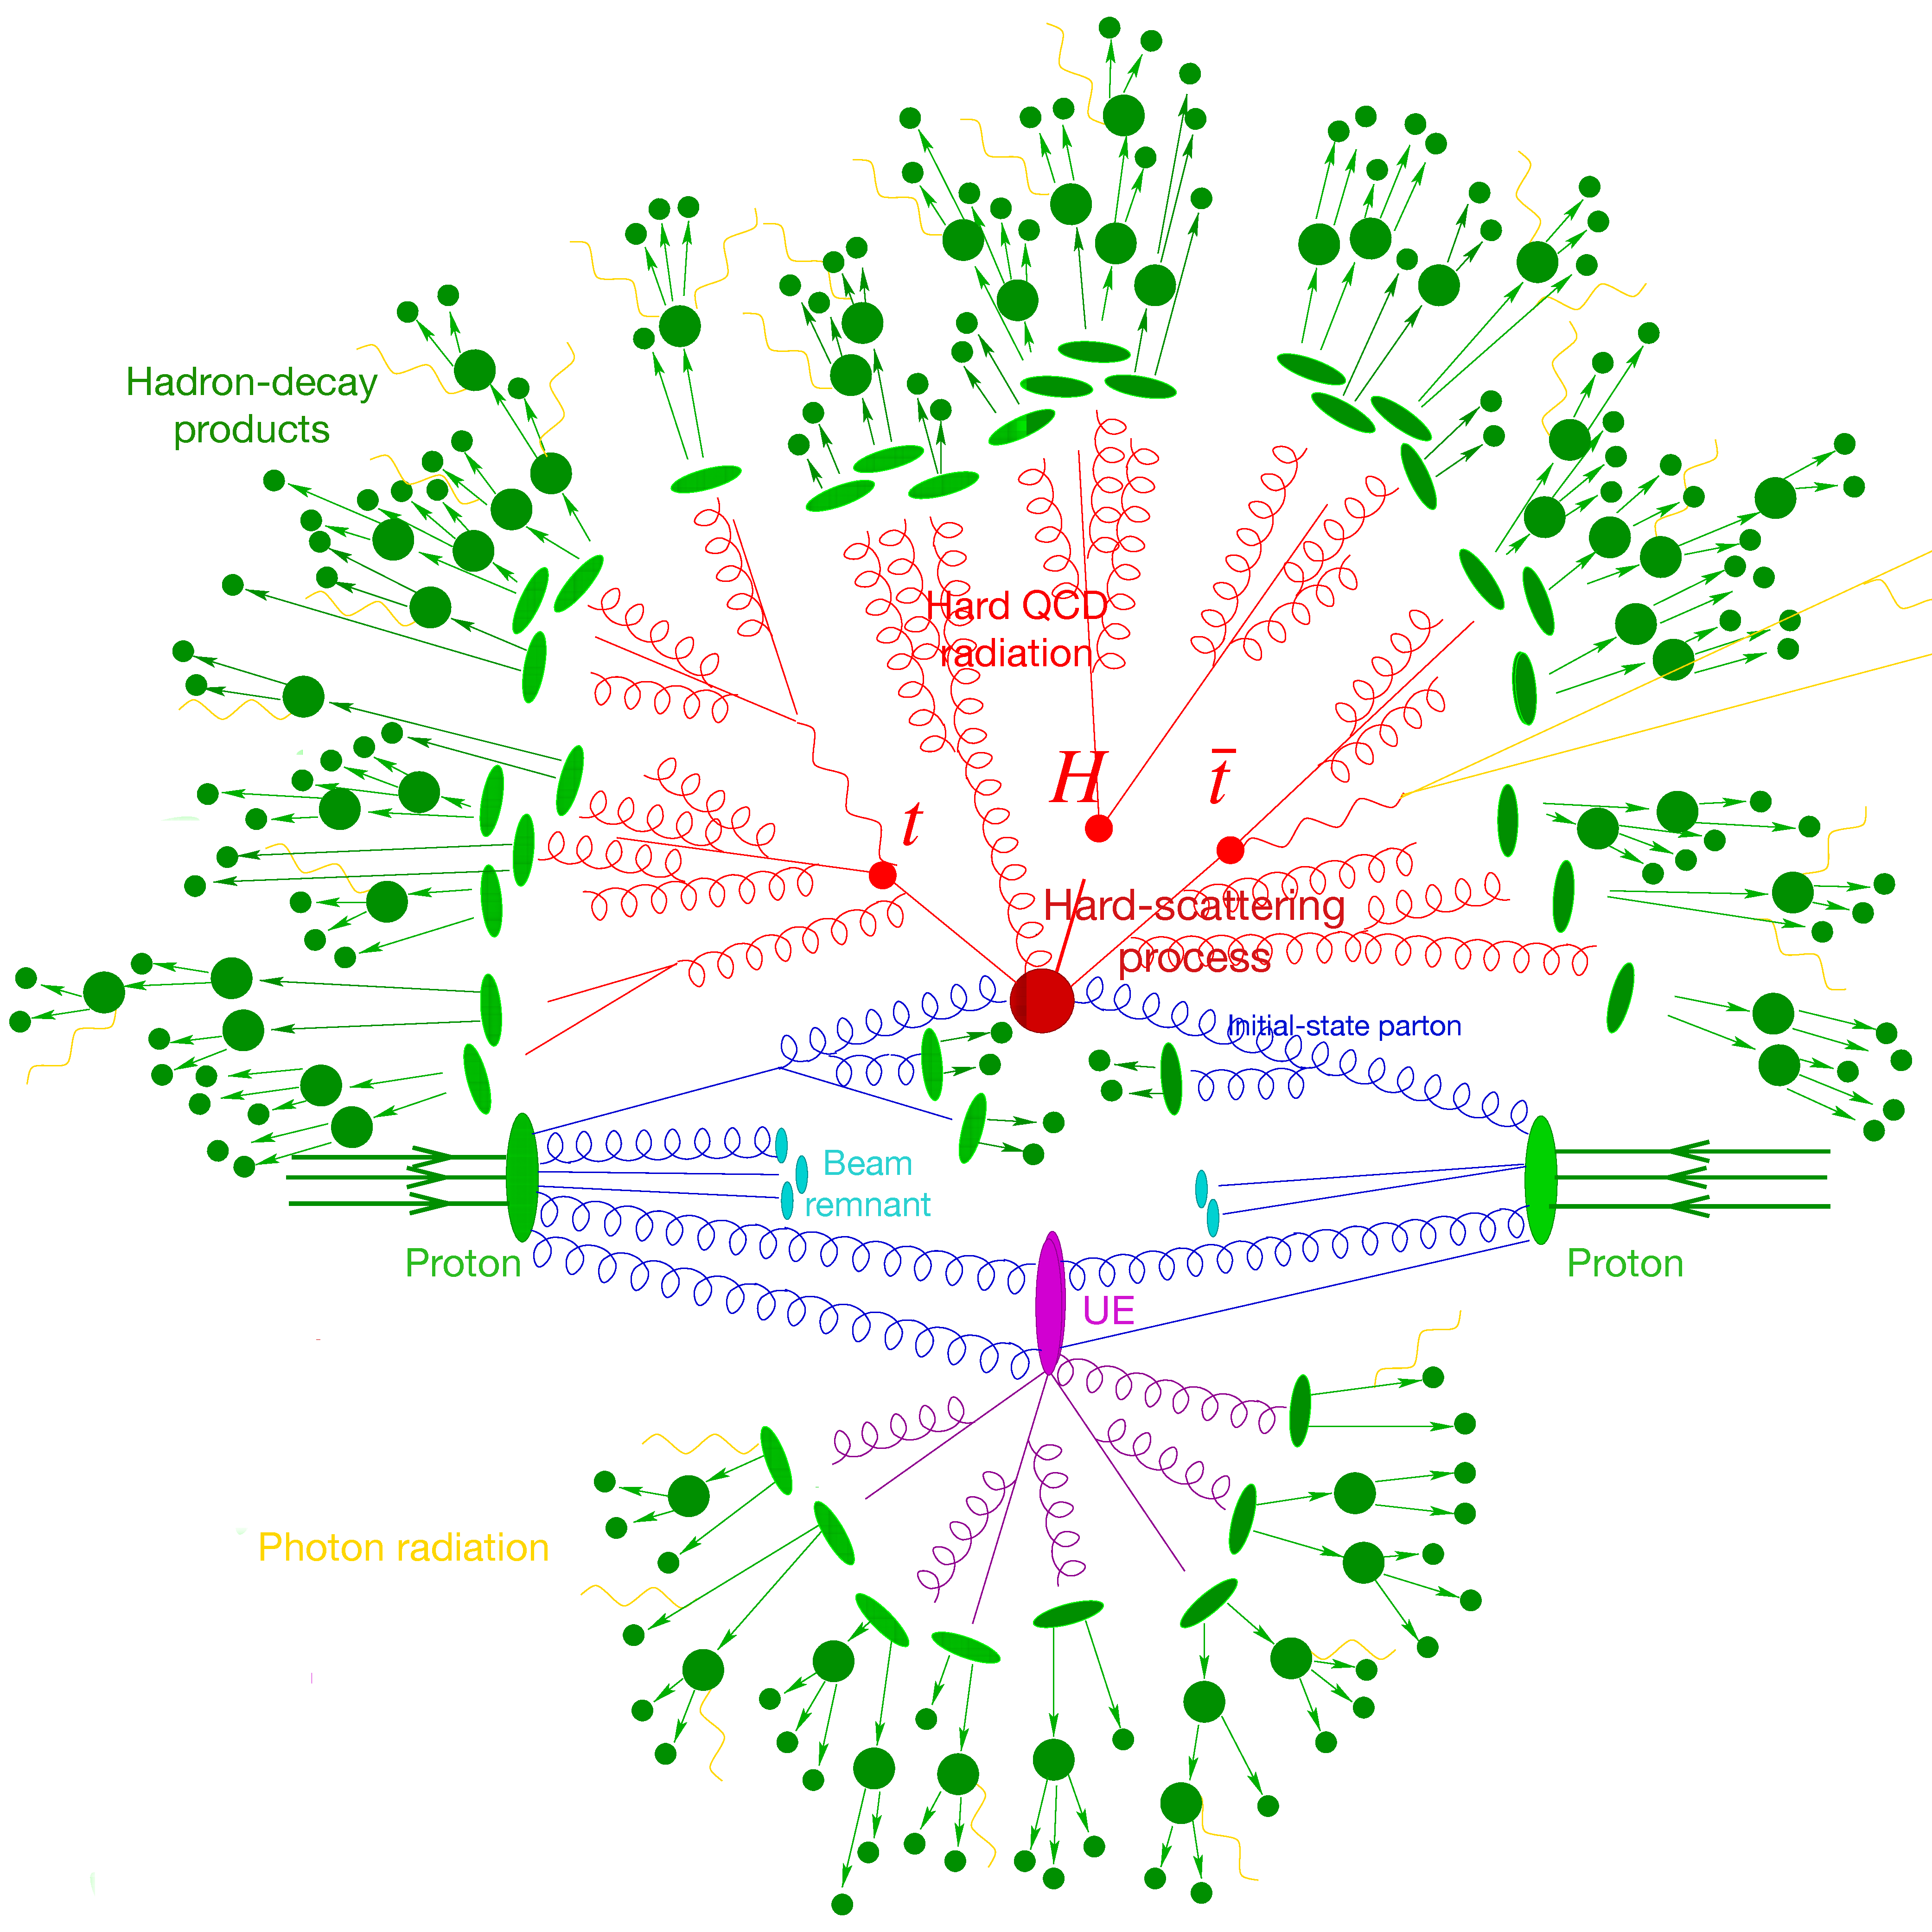
\includegraphics[width = \textwidth]{Chapter3/Generator_ttH_modified}
    \caption{Representation of a \ttH event from a $\Pproton \Pproton$ collision as produced by an event generator~\cite{Gleisberg:2008ta}. 
    The big red blob at the centre is the hard-scattering interaction, which produces the final state composed of the Higgs 
    boson and the two top quarks, represented by the three small red blobs. 
    The additional QCD radiation produced from these particles and the PS is also in red. 
    The secondary interaction, in purple, occurs before the formation of hadrons (in light green). 
    In darker green, the hadron decay is presented. The photon radiation can occur at any moment and appears in yellow.}
    \label{fig:Chap3:ttHSimulated}
\end{figure}



		
		
\subsubsection{Parton shower and hadronisation}
\label{sec:Chap3.1:MC:Steps:PS}

Once the hard-scattering process is simulated, the second step is to
incorporate corrections to account for additional radiations. 
Both the PS and the hadronisation are simulated by the event generator.  

\paragraph{Parton shower}\mbox{}\\
Parton showers are algorithms employed to simulate the soft radiation of 
gluons and quarks, collectively termed partons, during high-energy particle 
collisions. When quarks or gluons with high energy are produced post-collision, 
they can emit subsequent softer gluons as they traverse away from the IP

%A particle shower is a cascade of secondary particles produced when a high-energy particle interacts with matter.
%The first particle interacts with the material producing a secondary particle with less energy than the first one.
%The second particle does the same and, in each step, the particles produced are less and less energetic. For a single incoming particle, 
%this process can continue for thousands of iterations~\cite{grupen_shwartz_2008}. %An illustration of the
%EM and hadronic particle cascades is shown in Figure~\ref{fig:Chap2:ATLAS:PShoweringSim}.

%The PS models such additional radiations. %up to a certain 
%cutoff scale, beyond which hadronisation algorithms combine the remaining quarks 
%and gluons to form hadrons. 
All the incoming or outgoing partons are involved in the PS simulation.
If the particles have colour charge or electric charge can emit
QCD (i.e. gluons) or QED (i.e. photons) radiation, respectively.
This process generates hundreds of particles with 
varying energies and momenta spanning multiple orders of magnitude.
%because particles with electric or colour charge can emit either QED (i.e. photons) 
%or QCD (i.e. gluons) radiations. The PS simulation computes the terms of the 
%perturbative expansion in the strong coupling constant considering the gluons emissions.
%In high-energy inelastic-collisions involving hadrons, the particles with colour charge
%can emit radiation in form of QCD (i.e. gluons).  
%The  colour confinement leads to the 
%production of many additional partons that ultimately form hadrons. 
The PS algorithm mimics the remaining terms of the perturbative expansion 
in $\alpha_{s}$ by emitting gluons which will eventually split into more partons.

The PS can either be dipole-, angular- or 
\pT-ordered~\cite{Platzer:2011bc, Gieseke:2003rz}. 
For the first case, the divergent structure of QCD amplitude can be reproduced in 
dipole-like emissions without double counting the soft wide-angle emissions.
% Dipole ref: https://www.ncbi.nlm.nih.gov/pmc/articles/PMC6191001/
In the second case, the angle of emission with respect to the incoming parton is decreased in each step. 
For the third, the ordering variable is the module of \pT of the parton. 
The successive branching is stopped when a certain cut-off scale is reached.
While \Pythia uses the \pT-ordered PS, \Herwig has the possibility of using
the dipole- or angular-ordered shower (see Section~\ref{sec:Chap3.1:MC:Generators} for 
an overview on the MC generatos).


%Since fixed-order 
%calculations involving these partons are not feasible in hadron-collider experiments, 
%PS algorithms are employed to obtain results that approximate all higher-order corrections 
%due to real emissions in the hard-scattering event. 

%The output of \MGNLO or \POWHEGBOX is used as input for the PS
%generators.


\paragraph{Hadronisation}\mbox{}\\
As the PS evolves, the energy and momentum of the involved
particles decrease until reaching a point in which the confinement
occurs and hadrons are formed. The hadronisation happens
around $1$~GeV and combines the coloured partons into colour-neutral
hadrons~\cite{Hoche:2014rga}. The hadronisation is a non-perturbative process and, hence, 
QCD-inspired models are used to simulate it.
Hadronisation operates on the foundation of the parton--hadron duality
hypothesis~\cite{Azimov:1984np}. This entails that the exchange of momentum 
and quantum numbers at the hadron level should adhere to the same principles 
as observed at the parton level. Therefore, partons are joined together to form
hadrons according to their proximity and phase spaces. 

The two predominant theoretical models which are employed to calculate the hadronisation are:
%the Lund-string~\cite{Andersson:1983ia, Sjostrand:1986hx} and the 
%cluster~\cite{Borozan:2002fk} theoretical models:
\begin{itemize}
	\item \textbf{Lund-string model}~\cite{Andersson:1983ia, Sjostrand:1986hx}: 
		This model describes the colour interaction between quarks in terms 
		of strings. In the Lund-string model, when a quark and an antiquark are pulled apart, the 
		interaction between them can be visualised as a string. As they move further apart, 
		the potential energy in the string increases. When the energy of the string becomes 
		sufficient, it becomes energetically favourable to produce a new quark--antiquark pair 
		from the vacuum (process known as ``breaking'' of the string). When the string breaks, 
		it effectively splits into two new strings, each connecting a quark to an antiquark.
		In high-energy collisions such as the ones at the LHC, multiple strings can be formed, 
		leading to the production of many hadrons.
		%One of the model's strengths is its ability to provide a relatively simple and intuitive 
		%picture of the hadronisation process while being consistent with experimental observations.

	\item \textbf{Cluster model}~\cite{Borozan:2002fk}: The quarks and antiquarks in this alternative model, 
		instead of forming strings like in the Lund-string model, group together to form 
		colour-neutral ``clusters'' which are the precursor to hadrons. 
		Once these clusters are formed, they are decayed into hadrons.
		Light clusters typically convert directly into mesons (like pions). 
		Heavier clusters can undergo decays producing multiple hadrons.
\end{itemize} 

The most relevant event generators for PS and hadronisation within this analysis are \Herwig~\cite{Bahr:2008pv}, 
\Pythia~\cite{Sjostrand:2014zea}, and \Sherpa~\cite{Gleisberg:2008ta}. Here, the fragmentation models
are included as well with \Pythia using the Lund-string model, \Herwig using the cluster model and
\Sherpa being able to use both.

\begin{comment}
\subsubsection{Soft QCD components, decays and QED radiation}
\label{sec:Chap3.1:MC:Steps:soft}
Following the evolution of the PS, the event generation-process continues with the 
incorporation of soft-QCD phenomena, decays of unstable particles, and QED 
radiation. This encompasses the UE (described in Section~\ref{sec:Chap1:PhenoOfPP:UE}) 
generation and the hadronisation process, both of which are based on models that 
cannot be deduced from fundamental principles due to their occurrence at low scales, 
where the strong-perturbation series becomes unreliable. 
%To determine the model parameters, fits to experimental data are performed, 
%and the values are compiled in various tunes of the programmes.
\end{comment}

\subsubsection{Underlying event}
When a hard-scattering subprocess occurs, additional production of hadrons takes place. 
This production cannot be attributed to the showering of the coloured partons involved in the subprocess. 
The concept of UE encompasses various phenomena, 
including pile-up reactions, MPI, and the characteristics of the soft fragments of protons.
%The UE is throught to result from collisions among partons in the 
%incoming hadrons that are not directly participating in the hard subprocess. 
The parameters used to simulate the UE must be adjusted based on experimental data.
The UE can be generated using \Herwig, \Pythia or \Sherpa.




\subsubsection{Hadron decay}
\label{sec:Chap3.1:MC:Steps:HadronDecay}
The final stage before introducing the detector geometry in event generation involves 
the decay of unstable hadrons.  
These hadrons can be produced in excited and unstable states during hadronisation 
and can subsequently decay into lighter, stable particles that can be detected within 
the range of the acceptance of the detector. A particle is considered unstable if 
its lifetime ($\tau_{\text{Particle}}$) satisfies $c\tau_{\text{Particle}} < 10$~mm. 

The experimental data suggest that many of the detected final-state particles 
originate from the decay of excited hadronic states. Therefore, most of the decays 
detailed in the Review of Particle Physics~\cite{Workman:2022ynf} should 
be considered, along with their respective decay patterns.
The high complexity of modelling and implementing 
this arises from the multitude of potential particles and decay chains involved.

\begin{comment}
\subsubsection{\P tau decay}
Given the short lifetime of the \Ptau lepton 
($2.9 \times 10^{-13}$~s), it is also considered unstable and, hence, its decays are generated 
within the MC event simulation chain. The matrix elements of the \Ptau decay are
integral part of the simulation chain.

\subsubsection{Top-quark and Higgs-boson decay}
The decay of the top quark and the Higgs boson is also a fundamental 
Done with madspin <- this conserves the spin information which is not explicitly used in
the \tHq search but it is relevant for other top analyses such as the measure of polarisation.
\end{comment}


%\paragraph{QED radiation}\mbox{}\\
%The effects of QED radiations from charged particles are also included in the MC generators.

\subsubsection{Pile-up}
\label{chap:DataAndMC:pileup}
The effects of the pile-up have to
be simulated as well. This phenomenon is modelled 
by overlaying over the original hard-scattering event with
inelastic $\Pproton \Pproton$ collisions. 
To do so in the ATLAS experiment, \PYTHIA[8] is 
used to generate
the minimum-bias events in the pile-up, i.e. events with low-momentum transfer. 

After this is done, the MC-generated events are weighted to 
reproduce the pile-up distribution provided by the LHC (see Figure~\ref{fig:Chap2:LHC:PileUp_15-18}).
%<$\mu$> observed in the real data registered at the ATLAS detector. 

\subsubsection{Simulation of the ATLAS detector, digitisation and reconstruction}
\label{sec:Chap3.1:MC:Steps:Reco}
The event simulation described so far refers to the generation of physical 
processes based only on the models. At this stage of the simulation chain, 
no information about any detector is included yet. %the
%events are referred to as ``particle-level'' events.

In order to compare the simulated data events\footnote{Although 
in this document are used the 
terms ``real detector data'' and ``MC simulated data'', it is usual to refer to these 
as ``data'' and ''simulation'', respectively.}.  with the real data
collected by ATLAS, the response of the detector has to be simulated. 
This includes the interaction of the many hundreds of particles present
in each event with the detector material, as the electronic output of the detector. 

To do so and as previously mentioned, the \GEANT toolkit is used to simulate the passage of 
the generated particles through the detector. Taking into account the geometry of the ATLAS detector,
 \GEANT simulates the effects of both, the magnetic fields and 
the detector material. Examples of these interactions are energy losses, multiple
scattering or photon conversions as well as the hits in the responsive material or interactions
with the non-sensitive material.

Afterwards, the electronic signal of the response of each detector is simulated too. This
step is known as digitisation and it is performed within Athena framework. %~\cite{Rebuzzi:2007maa}
The ATLAS digitisation software transforms the hits generated 
by the primary simulation (from the hard scattering to the interaction with the detector material) 
into responses of the detector named ``digits''.
A digit is generated when the voltage or current on a specific readout channel
of a detector surpasses a predetermined threshold within a certain time frame.
% Depending on the subdetector, the digit format might capture the precise signal 
% shape over this period, while others might only note that the threshold was surpassed 
% during the designated time window.
The detector noise is added in this step.
The simulated digital output is used to 
reconstruct the physical objects of the MC event. The reconstruction procedure is 
done identically for real data and generated simulation. % and it is described in
%Chapter~\ref{chap:ObjectReconstruction}. 
Before performing the
digitisation the triggers are simulated as well.

The MC events that have undergone the complete simulation chain 
are designated as ``reconstruction-level'' events. Later, for the
lepton-origin assignment (Section~\ref{sec:ChaptH:Sig:LepAsign})
these denominations are used when comparing the information of 
a single event at different levels.

\paragraph{Full and fast simulations of the ATLAS detector}\mbox{}\\
%\paragraph{Atlfast-II and ATLAS full simulation}\mbox{}\\
A meticulous simulation of the response of the ATLAS detector
is of paramount importance to obtain accurate results.
Nevertheless, given the high collision rate that takes
place within the LHC experiments, conducting a comprehensive full-detector simulation
considering all the events presents significant challenges and can 
be computationally intensive.
In some instances, the use of a simplified and fast approach is 
enough for the analysis. Hence, there are two proposed 
detector MC simulation techniques: Full Simulation (FS)~\cite{SOFT-2010-01} and Atlfast-II Fast 
Detector Simulation (AFII)~\cite{ATLAS:2010bfa, SOFT-2010-01}.

The FS strategy relies on a complete % FS = complete ATLAS detector simulation
detector description powered fully by the \GEANT toolkit. %\cite{ATLAS:2010arf, GEANT4:2002zbu}. 
This thorough simulation demands extensive CPU processing time for each event, 
especially within the calorimeters. 
Alternatively, the AFII strategy considers 
a parametrised cell response to simulate
the particle-energy response and the energy distribution in the ATLAS calorimeter~\cite{ATLAS:2010bfa, Yamanaka:2011zz}.
This allows AFII to deliver a valid and good-performing simulation within the computing limits of the collaboration.
For the ID and the MS, AFII uses the full \GEANT simulation.

\subsection{MC generators}
\label{sec:Chap3.1:MC:Generators}
The different steps employed in the event simulation chain make use of various
MC event generators. The most relevant ones for this thesis are mentioned here.
Later, on Section~\ref{sec:ChaptH:Data_and_MC}, the specific generator for
each simulated sample are presented.

\begin{itemize}
	\item \textbf{\MGNLO}: Short for ``Matrix element Automatic Generator'', is a NLO
		generator for producing the $\mathcal{M}$ for events following 
		various schemes (e.g.
		$2 \rightarrow 1$, $2 \rightarrow 2$, $2 \rightarrow 3$ or $2 \rightarrow 7$). %2->7 is used for ttgamma
		These schemes correspond to the multiplicity of initial and final particles
		in the Feynman diagram. For instance, the $2 \rightarrow 2$ and $2 \rightarrow 3$
		correspond, respectively, to the 5FS and 4FS described
		in Section~\ref{sec:Chap1:tH:ProductionModes}.
		Given the process, \MGNLO automatically creates the $\mathcal{M}$  for all the 
		subprocesses and produces the mappings for the integration over the phase space. 
		After this step, the event can be transferred to a PS generator such as \Herwig or \Pythia.
		%The first refers to a scattering event where two particles come in and one goes out.
		%The second (and third), denote interactions where two 
		%incoming particles produce two (three) outgoing particles.
		%\MGNLO produces the simulations in the ``Les Houches'' format.
		% Some events are generated with negative weights due the one loop corrections included
		% but any resulting distribution will be physical (i.e. positive) if enough statistics are available.
		% Later on, when the BDTs are trained, this supposes a nuisance as it is
		% described in Section~\ref{sec:ChaptH:Sig:LepAsign:SS:BDT:NegWeights}.
		
	\item \textbf{\POWHEGBOX}: Short for ``Positive Weight Hardest Emission Generator'', it is
		another NLO generator based on the $\mathcal{M}$ following various schemes 
		(e.g. 5FS, 4FS o $2 \rightarrow 4$ ). % 2 -> 4 for bb4l
		Here, the 
		$\mu_{\text{R}}$ and $\mu_{\text{F}}$ are set to be equal to the \pT of the hard partons.
		%Its basic idea is to generate the hardest radiation 
		%first, and then feed the event to any shower generator for subsequent, softer radiation.
		%In principle, 
		This generator was built to implement the same physics as \MGNLO but
		outputting positively weighted events only and, hence, escaping the challenge of
		dealing with negatively-weighted events. Nevertheless, in some cases, the negative weights
		appear in the generation with (e.g. \tchannel process)~\cite{Alioli:2010qp}.
		% 	POWHEG :: El aglorítmo.
		%	POWHEG BOX :: El generador. 

	\item \textbf{\Herwig[7]}~\cite{Bahr:2008pv, Bellm:2015jjp}: Its name comes from ``Hadron Emission Reactions With Interfering Gluons''.
		This flexible generator has a huge diversity of QCD processes which includes $\mathcal{M}$ 
		and PS simulation at LO and NLO. Even though it can generate the hard-scattering process, in
		the analysis carried in this thesis it is employed for PS simulation. 
		By default, the PS is ordered 
		using either angular- or 
		dipole-ordered distribution (the default is angular). \Herwig[7] makes use of the cluster model for hadronisation, 
		and an eikonal multiple-interaction model for UE~\cite{Borozan:2002fk}. 
		% eikonal = https://arxiv.org/pdf/hep-ph/0207283.pdf
		
	\item \textbf{\Pythia[8]}~\cite{Sjostrand:2007gs, Sjostrand:2014zea}: 
		Based on $\mathcal{M}$ at LO, this general-purpose
		event generator implements
		various calculations (e.g. $2 \rightarrow 1$ and $2 \rightarrow 2$).
		Contrary to \Herwig, the ISR and FSR are matched in \pT-ordered in the PS. 
		% https://arxiv.org/pdf/1005.4568.pdf (3.4.1)
		Regarding the hadronisation, \Pythia[8] uses the Lund-string model.
		It can also compute the UE using a multiple-interaction model~\cite{Sjostrand:1987su}.
		Most of the PS 
		and \pileup in this analysis are
		simulated using \Pythia[8]. %As it is presented on Section~\ref{sec:ChaptH:Data_and_MC:MC},
		%It includes support for both ``Les Houches'' and ``HepMC'' event formats.
		%This generator is frequently used in the simulation of minimum-bias events. 
		% Pythia 8 <-
		
	\item \textbf{\Sherpa}~\cite{Gleisberg:2008ta, Sherpa:2019gpd}: 
		Standing from ``Simulation of High-Energy Reactions of Particles''.
		It is designed to provide a comprehensive approach to the simulation of particle collisions, 
		like \Herwig and \Pythia, %In contrast to the others, SHERPA presents a modular design, 
		%aspects or phases of a collision, into a cohesive whole. 
		being able to simulate from the $\mathcal{M}$ of the hard-scattering process to the PS and hadronisation.
		For the hard scattering, the events can be constructed with $2 \rightarrow 2$  processes. 
		%The PS is based phenomenological cluster-hadronisation, while a multiple-interaction 
		%model is used for the UE.
		The PS is based on the Lund model and it is interfaceable with \Pythia[8].
		%It is expected to give better approximations for final states with large numbers of isolated 
		%jets than the previous methods.
		
	\item \textbf{\MADSPIN}~\cite{Frixione:2007zp, Artoisenet:2012st}:
		This generator considers the generation of NLO events involving heavy resonances.
		In this thesis, the processes with a single top quark are decayed at LO using this generator because
		it preserves spin correlations.
	\item \textbf{\EVTGEN}~\cite{Lange:2001uf}: This MC event generator simulates the decays of 
		heavy flavour hadrons, primarily $B$, and $D$-type mesons. It contains a range of decay 
		models for intermediate and final states containing scalar, vector and tensor mesons or 
		resonances, as well as leptons, photons and baryons.
\end{itemize}

\begin{comment}


Several MC event-generator programs use the general features outlined above
to imitate the experimental data. This thesis uses the most common generators. 
This section provides a description of these. The MC generators implemented include:

% GENERATORS:
%      MadGraph5_aMC@NLO 2.6.2
%      MadGraph5_aMC@NLO 2.3.3
%      MadGraph5_aMC@NLO 2.8.1
%      Powheg Box v2
%      Powheg Box v1
%      Sherpa 2.2.1
%      Sherpa 2.2.1-2
%      Sherpa 2.2.2
%      Sherpa 2.2.10
%      Pythia 8.186


% PARTON SHOWER:
%      Pythia 8.230
%      Pythia 8.210
%      Pythia 8.186
%      Pythia 8.245p3

\begin{itemize}
	\item \MGNLO is employed for the matrix element in the event generation
	\item \POWHEGBOX is also employed for the matrix element in the event generation
	\item \SHERPA
	\item \PYTHIA[8] takes the output of \MGNLO or \POWHEGBOX~\cite{Frixione:2007vw} to simulate the PS.
				is is a C++ code. 
	\item \HERWIG for alternative PS samples
\end{itemize}
\end{comment}






%POSTAMBLE
\begin{comment}
asdf
%\end{document}
%ENDPOSTAMBLE
\end{comment}
